\section{Why firms merge and how mergers are reviewed}\label{sec:11-motives}

A horizontal merger removes the competition between the merging firms and may let them produce more cheaply.
Whether consumers gain or lose depends on which force dominates, and on how rivals respond. This section
describes how often firms merge, why they do so, and how a proposed merger is reviewed in the United States. \Cref{sec:11-marketdef} turns to the screens that
the agencies apply first, and \cref{sec:11-cournot} develops the theory of mergers in homogeneous-goods markets.

\subsection{Merger activity and merger waves}\label{sec:11-waves}

Mergers are frequent, and their total value is large. \Cref{fig:11-waves} shows the number and value of
mergers and acquisitions worldwide since 1985. The number of deals trends upward fairly smoothly. Their value
moves in \emph{waves}, periods in which deal values rise quickly and then collapse. Values peak around 1999 and
2000, in 2007, in 2015 and in 2021, and they reach troughs around 2002, 2009 and 2023. The highlighted year,
1997, saw 26,227 transactions worth \$1,824 billion. The last two entries are not full-year data. One covers
January to March 2026, and the other is a projection for the whole of 2026.

\begin{figure}[htbp]
\centering
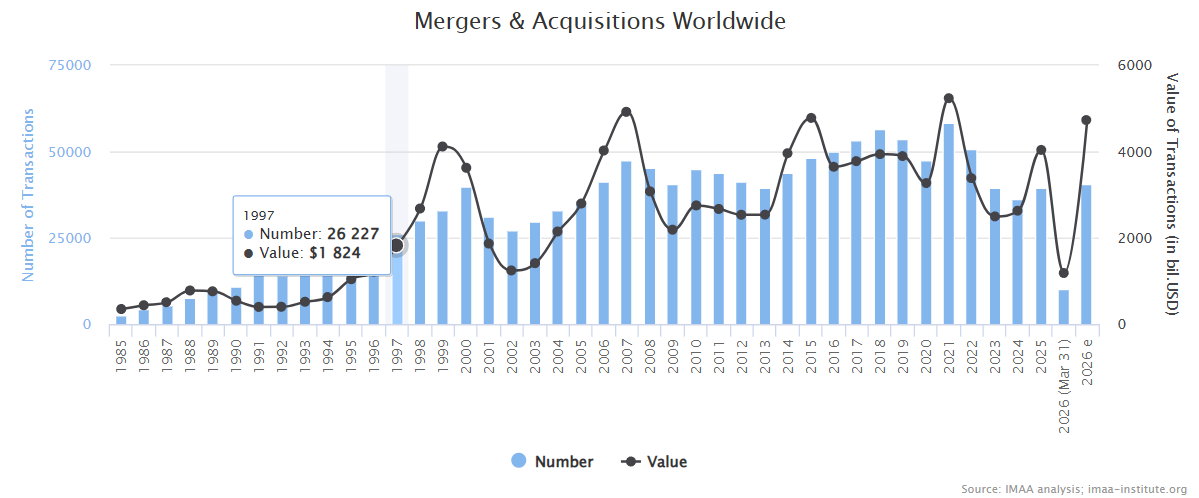
\includegraphics[width=\textwidth]{figures/ch11/mna_waves.png}
\caption{Number of transactions (bars, left axis) and value of transactions in billions of US dollars (line,
right axis) of mergers and acquisitions worldwide, 1985--2026. The 2026 entries are the first quarter and a
full-year estimate. Source: Institute for Mergers, Acquisitions and Alliances (IMAA), imaa-institute.org.}
\label{fig:11-waves}
\end{figure}

Within an industry, mergers often come in sequences that reshape the market over two or three decades.
\Cref{tab:11-consolidation} summarizes three such histories. US telecommunications went from the 1984 breakup of
AT\&T into seven regional ``Baby Bells'' to a handful of national carriers. The major US airlines consolidated
through mergers and failures after deregulation (\cref{ch:airlines}). World brewing was transformed by a chain of
very large deals between 2000 and 2012, and \cref{sec:11-millercoors} studies one of them, the MillerCoors joint
venture, in detail. \Cref{fig:11-beer} reproduces the brewing timeline.

\begin{table}[htbp]
\centering
\caption{Three consolidation histories}
\label{tab:11-consolidation}
\footnotesize
\begin{tabularx}{\textwidth}{@{}p{2.0cm}X@{}}
\toprule
Industry & Main combinations and outcome \\
\midrule
US telecom &
In 1984 AT\&T's local operations were split into seven regional companies: Ameritech, Bell Atlantic,
BellSouth, NYNEX, Pacific Telesis, Southwestern Bell and U\,S West. Southwestern Bell, renamed SBC, absorbed
Pacific Telesis (1997) and Ameritech (1999), then acquired AT\&T Corp.\ (2005) and took the name AT\&T Inc.,
and then acquired BellSouth (2006). Bell Atlantic, NYNEX and GTE formed Verizon (2000), which later absorbed MCI,
while Verizon Wireless absorbed Alltel. Qwest absorbed U\,S West and was in turn absorbed by CenturyLink.
Subscribers at the end of 2010 were: AT\&T 24 million landline and 96 million wireless, Verizon 26 million
landline and Verizon Wireless 94 million. Sprint had 50 million, T-Mobile USA 34 million and CenturyLink 15 million
landline. AT\&T's proposed \$39 billion purchase of T-Mobile USA (2011) was abandoned the same year
(\cref{tab:11-recent}). \\[3pt]
US airlines &
After deregulation in 1978, Trans World Airlines (which had absorbed Ozark) was acquired by American (2001).
Republic Airlines, itself formed from North Central, Southern and Hughes Airwest, merged into Northwest, and
Northwest merged into Delta (2008), which had absorbed Western (1987). Continental, which had absorbed People
Express among others, merged with United (2010). US Airways merged with America West (2005) and later with
American (2013). Southwest absorbed AirTran (2011). Braniff (1982), Eastern (1991) and Pan Am (1991) failed. \\[3pt]
World beer &
Interbrew and AmBev (\$11.5 billion) formed InBev (2004), which bought Anheuser-Busch for \$52 billion (2008)
to form AB InBev and later bought the rest of Grupo Modelo for \$20.1 billion. SAB bought Miller (\$5.6 billion,
2002) and later Bavaria, Grolsch and Foster's. Coors and Molson merged (2005). Heineken and Carlsberg divided the
assets of Scottish \& Newcastle (\$15.3 billion, 2008). In the United States, SABMiller and Molson Coors combined
their operations in the MillerCoors joint venture (2008). \\
\bottomrule
\end{tabularx}

\vspace{3pt}
\begin{minipage}{\textwidth}
\footnotesize Notes: Subscriber counts and the T-Mobile deal value are from a 2011 \emph{Wall Street
Journal} graphic (``A Tangled Family Tree''). Airline combinations follow the Aviation Week Intelligence
Network's Fleet Database as reproduced in the source chart, and beer deal values follow the timeline of
\cref{fig:11-beer}. Years are completion years, except the year of the proposed T-Mobile purchase. The telecom
and beer years, Western (1987) and the three airline failures are read off the time axes of these charts. The airline mergers of 2001 to 2011 are dated by
\citet[p.~11]{GAO2013}, and the 2013 merger of American and US Airways by \citet[p.~263]{AskerNocke2021}. MillerCoors
is dated by its consummation in June 2008 \citep[p.~1768]{MillerWeinberg2017}.
\end{minipage}
\end{table}

\begin{figure}[htbp]
\centering
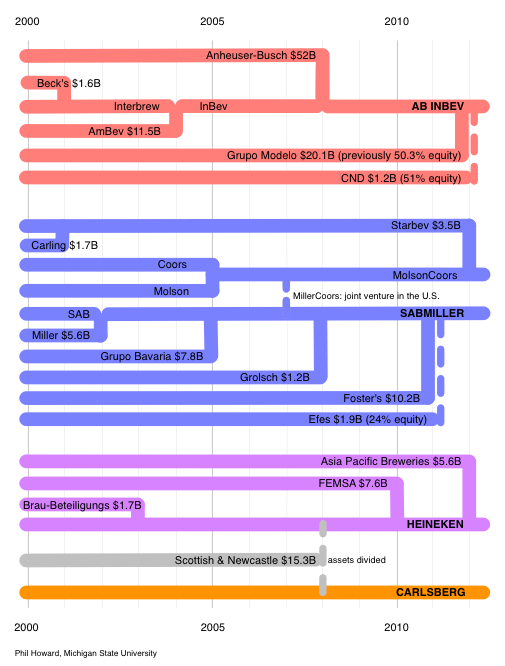
\includegraphics[width=0.5\textwidth]{figures/ch11/beer_timeline.png}
\caption{Consolidation of the world beer industry, 2000--2012. Each band is a brewer, and a band that ends in
a vertical connector is acquired by the band it joins. Labels give deal values in billions of US dollars.
Source: Phil Howard, Michigan State University, as printed on the figure.}
\label{fig:11-beer}
\end{figure}

\casehead{Two views of why firms merge}
Industrial organization economists stress three motives. The first is market power. A merger internalizes the
competition between the merging firms, which gives them a reason to raise prices even if all other firms keep
competing as before. These are the unilateral effects defined in the introduction to this chapter. A merger may
also make it easier for the remaining firms to coordinate, tacitly or explicitly, which gives rise to coordinated
effects (\cref{ch:collusion-theory}). The second motive is efficiencies. They include economies of scale and scope,
the rationalization of production and distribution across plants, and the transfer of know-how from the better-run
firm to the other. The third motive is strategic. A merger can deter entry or allow the firms to reposition their
products.

Corporate finance asks different questions. One is why mergers come in waves and why they cluster within
industries. \citet{MitchellMulherin1996} and \citet{AndradeMitchellStafford2001} attribute the clustering to
industry shocks, such as deregulation, new technologies and changes in input prices, which make a new industry
structure efficient. A second question is why the stock returns of acquirers are weak around acquisitions while
targets gain. Several theories blame agency problems or mispricing. \citet{Jensen1986} argues that managers of
firms with free cash flow overinvest in acquisitions to build empires. \citet{Roll1986} argues that overconfident
managers overpay. \citet{ShleiferVishny2003} argue that overvalued acquirers use their stock to buy undervalued
targets, so that waves follow stock-market valuations. These explanations are complements to the industrial
organization view and say little about prices. We therefore leave them aside.

The theory developed in this chapter delivers three results that will guide the empirical work. In a Cournot
market, a merger without cost savings raises the price, and it is often unprofitable for the merging firms
(\cref{sec:11-cournot}). In a symmetric market with differentiated products and price competition, every merger
is profitable (\cref{sec:11-upp}). When firms must invest in costly capacity, a merger can be profitable even
without cost savings (\cref{sec:11-beyond}).

\subsection{The legal framework and the US review process}\label{sec:11-review}

Section 7 of the Clayton Act of 1914, as amended in 1950, prohibits acquisitions whose effect ``may be
substantially to lessen competition, or to tend to create a monopoly'' \citep[p.~2]{FarrellShapiro2010}. The
word ``may'' matters. The government does not have to prove that a merger will harm competition, only that it is
likely to. Section 7 applies to every acquisition, including those that are too small to be reported and those
already consummated.

\casehead{Notification and the waiting period}
The Hart-Scott-Rodino Antitrust Improvements Act of 1976 (HSR) added Section 7A to the Clayton Act. It requires
the parties to a sufficiently large transaction to notify the Federal Trade Commission (FTC) and the Antitrust
Division of the Department of Justice (DOJ) before they close. Its motivation was the cost of undoing completed
mergers. The leading example, \emph{United States v.\ El Paso Natural Gas}, took seven years to litigate and ten
more years to carry out the divestiture the Supreme Court had ordered \citep[p.~5]{AshenfelterHosken2008}. Until
2001 every merger involving more than \$15 million in assets had to be reported. In February 2001 the threshold
rose to transactions above \$50 million and was indexed to the growth of national income, which explains much of
the fall in filings after 2001 \citep[p.~6, n.~7]{AshenfelterHosken2008}. The indexed threshold was \$63 million
in 2008 \citep[p.~2, n.~3]{FarrellShapiro2010} and \$133.9 million in 2026 \citep[p.~2134]{FTC2026}. The 2001
change also altered which mergers took place, as the end of this subsection shows.

After both parties file, a waiting period of 30 days begins (15 days for cash tender offers and bankruptcy
sales). During this period the two agencies decide which one will review the deal, a step called
\emph{clearance}. That agency then conducts a preliminary review of market shares, concentration, company
documents and complaints from customers or rivals. The agency may end the wait early through \emph{early
termination}. If the deal looks problematic, the agency issues a \emph{Second Request}, a detailed subpoena for
documents and data on competition, entry, substitution and claimed efficiencies. The waiting period then extends
until 30 days after the parties have substantially complied \citep[p.~6]{AshenfelterHosken2008}. Compliance
typically takes two or three months and sometimes six months or more. The whole investigation, with depositions
and interviews of customers and competitors, often lasts about a year.

\casehead{Outcomes}
An investigation ends in one of four ways. The agency may close it and let the merger proceed. It may negotiate
a \emph{consent decree}, usually requiring the parties to divest overlapping assets. For DOJ decrees, the Tunney
Act requires a federal court to find that the decree is in the public interest. The agency may sue to block the
merger, which in practice means seeking a preliminary injunction in federal court. Finally, the parties may
abandon the deal. The last three outcomes are counted as \emph{enforcement actions}. Much of the bargaining takes
place in the shadow of litigation. In fiscal year 2006, for example, 1,768 transactions were reported, the
agencies issued 45 Second Requests and challenged 32 transactions. The challenges led to 17 settlements, 6
restructured transactions and 9 abandoned deals \citep[p.~2, n.~5]{FarrellShapiro2010}. Some industries follow
their own rules. Rail mergers, for instance, fall under the exclusive jurisdiction of the Surface Transportation
Board. \Cref{fig:11-hsrflow} summarizes the process.

\begin{figure}[htbp]
\centering
\begin{tikzpicture}[
  box/.style={draw, rounded corners=2pt, align=center, font=\footnotesize, text width=2.2cm,
              minimum height=1.05cm, inner sep=3pt, execute at begin node={\hyphenpenalty=10000\exhyphenpenalty=10000}},
  proc/.style={box, fill=gray!8},
  dec/.style={box, fill=yellow!14},
  pass/.style={box, fill=green!9},
  stopb/.style={box, fill=red!9},
  arr/.style={-{Stealth[length=2mm]}, thin},
  lab/.style={font=\scriptsize, inner sep=1.5pt}]
\node[proc] (agree) at (0,0) {Firms agree to merge};
\node[dec]  (rep)   at (3.05,0) {Reportable under HSR? (deal above threshold)};
\node[proc] (file)  at (6.1,0) {Both parties file, FTC or DOJ takes the case};
\node[proc] (rev)   at (9.15,0) {30-day review: shares, HHI, documents, complaints};
\node[dec]  (sr)    at (12.2,0) {Second Request?};
\node[pass, text width=2.6cm] (notrep) at (3.05,-2.45) {Not reportable: close at will, still subject to
  Clayton Act Section 7};
\node[pass, text width=3.0cm] (wait) at (8.2,-2.45) {Waiting period ends, or early termination,
  then close};
\node[proc, text width=3.4cm] (deep) at (12.2,-2.45) {In-depth investigation: data, documents,
  diversion, UPP, simulation (often about one year)};
\node[pass, text width=2.3cm]  (o1) at (5.4,-5.0)  {Close investigation};
\node[proc, text width=2.3cm]  (o2) at (8.0,-5.0)  {Consent decree: divest overlaps};
\node[stopb, text width=2.3cm] (o3) at (10.6,-5.0) {Sue to block (injunction in federal court)};
\node[stopb, text width=2.3cm] (o4) at (13.2,-5.0) {Parties abandon};
\draw[arr] (agree) -- (rep);
\draw[arr] (rep) -- node[lab, above] {yes} (file);
\draw[arr] (rep) -- node[lab, right] {no} (notrep);
\draw[arr] (file) -- (rev);
\draw[arr] (rev) -- (sr);
\draw[arr] (sr.south west) -- (wait.north east);
\node[lab, anchor=north east] at (9.95,-1.15) {no (about 98\%)};
\draw[arr] (sr) -- node[lab, right] {yes (about 2\%)} (deep);
\foreach \o in {o1,o2,o3,o4} {\draw[arr] (deep.south) -- (\o.north);}
\draw[decorate, decoration={brace, mirror, amplitude=5pt}] ([yshift=-3pt]o2.south west) --
  node[below=6pt, font=\footnotesize] {enforcement actions} ([yshift=-3pt]o4.south east);
\end{tikzpicture}
\caption{From the decision to merge to closing in the United States. In fiscal year 2025 there were 2,006 HSR
filings, 41 Second Requests and 18 enforcement actions, equal to 2.0 and 0.9 percent of filings. Two of the 18
actions concerned transactions not reported under HSR.}
\label{fig:11-hsrflow}
\end{figure}

\Cref{tab:11-hsr} reports the number of filings, Second Requests and enforcement actions in each fiscal year
from 2003 to 2025, and \cref{fig:11-hsrplot} extends the series back to 1991. Three patterns stand out. Filings
fell from 4,926 in fiscal year 2000 to 1,187 in 2002 after the threshold increase, and to 716 in fiscal year 2009
during the financial crisis. They spiked in 2021 and 2022. Over 2003--2025 the agencies issued 2.6 Second Requests
and brought 2.0 enforcement actions for every 100 filings. These are annual activity ratios. An action can concern a
transaction filed in an earlier year, or one that was never reportable. The ratio is therefore not the share of a
year's filings that led to enforcement. Actions relative to filings have drifted down, from about 3 percent in
2010--2013 to about 2 percent in 2014--2020 and between 0.9 and 1.6 percent since 2021. Most mergers are never
examined closely.

\begin{table}[htbp]
\centering
\caption{Hart-Scott-Rodino filings, Second Requests and enforcement actions, fiscal years 2003--2025}
\label{tab:11-hsr}
\footnotesize
\begin{tabular}{@{}lrrrrr@{}}
\toprule
 & & & & \multicolumn{2}{c}{Ratio to filings (percent)} \\
\cmidrule(l){5-6}
Fiscal year & Filings & Second Requests & Enforcement actions & Second Requests & Enforcement actions \\
\midrule
2003 & 1,014 & 33 & 36 & 3.3 & 3.6 \\
2004 & 1,454 & 35 & 24 & 2.4 & 1.7 \\
2005 & 1,675 & 50 & 18 & 3.0 & 1.1 \\
2006 & 1,768 & 45 & 32 & 2.5 & 1.8 \\
2007 & 2,201 & 63 & 34 & 2.9 & 1.5 \\
2008 & 1,726 & 41 & 37 & 2.4 & 2.1 \\
2009 & 716 & 31 & 31 & 4.3 & 4.3 \\
2010 & 1,166 & 42 & 41 & 3.6 & 3.5 \\
2011 & 1,450 & 55 & 37 & 3.8 & 2.6 \\
2012 & 1,429 & 49 & 44 & 3.4 & 3.1 \\
2013 & 1,326 & 47 & 38 & 3.5 & 2.9 \\
2014 & 1,663 & 51 & 33 & 3.1 & 2.0 \\
2015 & 1,801 & 47 & 42 & 2.6 & 2.3 \\
2016 & 1,832 & 54 & 47 & 2.9 & 2.6 \\
2017 & 2,052 & 51 & 39 & 2.5 & 1.9 \\
2018 & 2,111 & 45 & 39 & 2.1 & 1.8 \\
2019 & 2,089 & 61 & 38 & 2.9 & 1.8 \\
2020 & 1,637 & 48 & 43 & 2.9 & 2.6 \\
2021 & 3,520 & 65 & 32 & 1.8 & 0.9 \\
2022 & 3,152 & 47 & 49 & 1.5 & 1.6 \\
2023 & 1,805 & 37 & 28 & 2.0 & 1.6 \\
2024 & 2,031 & 59 & 32 & 2.9 & 1.6 \\
2025 & 2,006 & 41 & 18 & 2.0 & 0.9 \\
\midrule
Total & 41,624 & 1,097 & 812 & 2.6 & 2.0 \\
\bottomrule
\end{tabular}

\vspace{3pt}
\begin{minipage}{0.97\textwidth}
\footnotesize Notes: Compiled from the annual HSR reports of the FTC and DOJ. Enforcement actions combine the
merger challenges of both agencies as printed in each year's joint report, using the corrected report for 2022. The
FTC later raised its 2017 count from 21 to 23, which would give 41 for that year. A report counts an action in the
year of the agency's first public action. The action can concern a transaction filed in an earlier year or one not
reportable under HSR, as did two of the 18 actions in 2025. The ratios are counts divided by filings in the same
year, so they measure annual activity. The compiled table we draw on reports Second Request rates 0.1 point higher for 2017--2020
(2.6, 2.2, 3.0 and 3.0). It probably divides by the transactions for which a Second Request could be issued. The 2003 and 2004 rows coincide with \citet[Table 1]{AshenfelterHosken2008}, and the 2006 row with
\citet[n.~5]{FarrellShapiro2010}.
\end{minipage}
\end{table}

\begin{figure}[htbp]
\centering
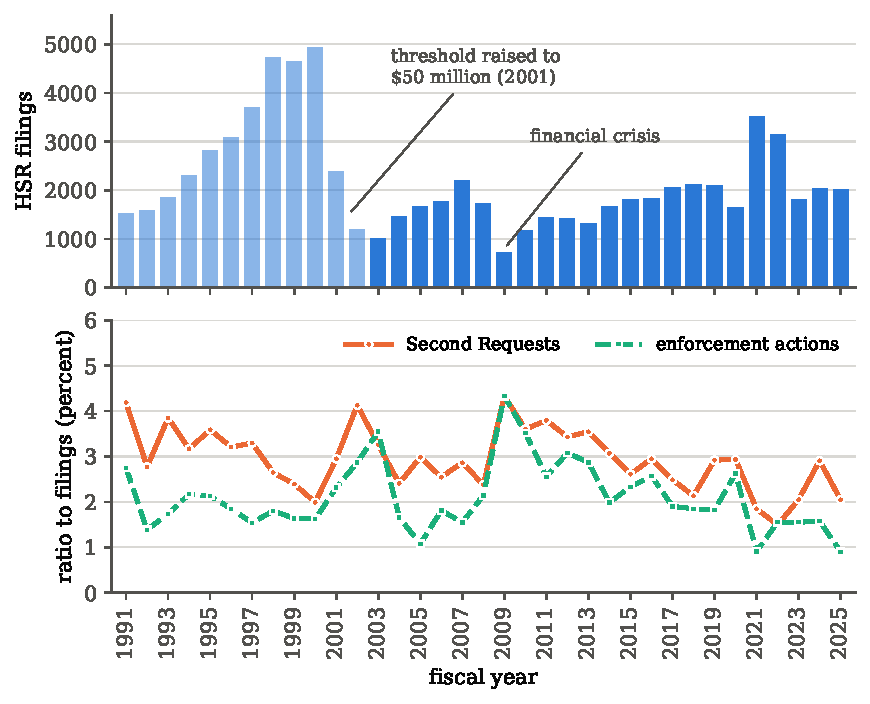
\includegraphics[width=0.86\textwidth]{figures/ch11/hsr_stats.pdf}
\caption{HSR filings (top) and the ratios of Second Requests and enforcement actions to filings in the same year, in
percent (bottom), fiscal years 1991--2025. The lighter bars for 1991--2002 come from \citet[Table 1]{AshenfelterHosken2008}, the
rest from \cref{tab:11-hsr}. Both ratios use all filings as the denominator.}
\label{fig:11-hsrplot}
\end{figure}

\casehead{Enforcement and selection}
Enforcement shapes which mergers we observe. \citet[p.~5]{AshenfelterHosken2008} report that 37,201 mergers were
filed from 1991 through 2004. About 97 percent were allowed to proceed without a full investigation. Of the 3
percent investigated in depth, roughly 65 percent were modified, abandoned or blocked.
\citet[p.~4, n.~5]{AshenfelterHoskenWeinberg2011} summarize the first figure as 97 percent of proposed mergers
going through without modification. Because the agencies try to stop the mergers most likely to raise prices,
the consummated mergers that a researcher can study are a selected sample. The average price effect of approved
mergers is a lower bound on the average effect that mergers would have in a world without enforcement
\citep{Carlton2009}. The informative object for policy is the effect of the \emph{marginal} merger, one that was
nearly blocked. \Cref{sec:11-retro} returns to this problem.

\casehead{Notification thresholds as a screen}
Reporting thresholds do more than save the agencies work. They also shape which mergers firms propose.
\citet{BesankoSpulber1993} model a review in which the merging parties know their merger-specific efficiencies and
the authority does not. Proposing a merger costs a fixed amount that cannot be recovered. Holding fixed the
probability of approval, only mergers whose efficiencies exceed a threshold are then worth proposing. A positive
proposal cost can therefore benefit consumers, because it improves the pool of proposed mergers
\citep[p.~223]{AskerNocke2021}. The same model suggests one reason why authorities apply a consumer surplus
standard rather than a total surplus standard. An authority that puts less weight on profit than society does is
tougher. It approves fewer mergers, and the proposals it receives are better as a result \citep[p.~223,
n.~120]{AskerNocke2021}.

\citet{Wollmann2019} tests this selection effect with the 2001 amendment, which raised the size-of-transaction
threshold. The agencies almost never investigated the newly exempt deals afterward, in line with the long-standing
observation that they rarely examine mergers that need not be reported. Wollmann compares newly exempt horizontal
mergers with newly exempt non-horizontal ones, which seldom raise concerns. This is a \emph{difference-in-differences}
design, which compares the change in a treated group with the change in a control group (\cref{sec:11-retro-problem}
develops it). A \emph{triple difference} also subtracts the same comparison among \emph{never-exempt} mergers, those
above the new threshold of \$50 million, which had to be reported both before and after the amendment. Newly exempt
mergers lie between the old \$15 million threshold and the new one. After
2001, never-exempt horizontal and non-horizontal mergers moved together. Newly exempt horizontal mergers rose
relative to newly exempt non-horizontal ones. The triple-difference estimate is a 50 percent increase: 324
additional newly exempt horizontal mergers per year on a pre-amendment base of 634 \citep[pp.~224--226]{AskerNocke2021}.
Through the lens of the Besanko-Spulber model, the amendment removed both the proposal cost and the risk of a
challenge for these deals. Mergers without large synergies became worth doing, so the pool of mergers grew and
worsened at the same time.

Firms also size their deals around the threshold. \citet{CunninghamEdererMa2021} study pharmaceutical acquisitions.
Acquisitions of targets whose drug projects overlap with the acquirer's bunch just below the HSR threshold, while
acquisitions without such overlap do not \citep[pp.~226--227 and Figure 9]{AskerNocke2021}. \Cref{sec:11-open}
returns to these acquisitions.

\subsection{What the agencies analyze}\label{sec:11-agencies}

The agencies' Horizontal Merger Guidelines describe five tasks \citep{USDOJFTC1992,USDOJFTC2010}, which
\citet[p.~7]{AshenfelterHosken2008} summarize. The first two
define the market. The \emph{relevant product market} is a set of close substitutes for the merging firms'
products, found with the hypothetical monopolist test of \cref{sec:11-hmt}. The \emph{relevant geographic market}
is the narrowest area in which anticompetitive effects could occur. For nationally distributed branded goods it is
typically the whole country \citep[p.~7]{AshenfelterHosken2008}. The third task is to assess competitive effects,
both unilateral and coordinated. The fourth is to evaluate efficiency claims. Efficiencies count only if they
are \emph{merger-specific}, meaning that no other arrangement that harms competition less could achieve them, and
\emph{verifiable} by the authority at the time of review \citep[p.~221]{AskerNocke2021}. They must also be large
enough to reverse the merger's potential to harm customers, for instance by preventing price increases
\citep[Section~10]{USDOJFTC2010}. The fifth is to ask whether entry would be timely, likely and sufficient to deter
or counteract the competitive effects of concern (Section~9). \Cref{sec:11-freeentry} shows what free entry implies
for the effects of a merger and how slowly entry can come in practice.
Economists at the agencies work mostly on market definition and competitive effects. The rest of this chapter
follows the same order. \Cref{sec:11-marketdef} covers market definition and concentration, and the remaining
sections cover competitive effects and efficiencies.

\casehead{Evidence on efficiencies}
The efficiency defense rests on a thin empirical base. \citet[pp.~219--221]{AskerNocke2021} single out two studies
that document merger-specific efficiencies. The first, \citet{AshenfelterHoskenWeinberg2015}, measures the
shipping savings of the MillerCoors joint venture, which \cref{sec:11-mc-assessment} discusses. The second,
\citet{BraguinskyEtAl2015}, studies 73 acquisitions in the Japanese cotton-spinning industry between 1896 and 1920.
More profitable firms bought less profitable ones, although the two groups had similar physical productivity. The
acquired mills then improved their inventory management, accounts receivable and capacity utilization, and market
power explains little of their higher profitability. The two cases illustrate the two conditions above. The beer
savings came from shorter shipping distances, which are easy to verify. The brewers might, however, have obtained
them by brewing each other's beer under contract while pricing independently, which questions their merger
specificity. The managerial gains in cotton spinning are specific to the merger but hard to verify before they
occur.

Evidence on how often mergers create efficiencies, and how large they are, is scarcer still.
\citet{GeurtsVanBiesebroeck2019} find that about 80 percent of the mergers in Belgium between 2005 and 2012 raised
employment, which may reflect higher output. \citet{GriecoPinkseSlade2018} estimate returns to scale in the
Molson-Coors merger and translate them into marginal-cost reductions \citep[pp.~221--222]{AskerNocke2021}. In the
words of \citet[p.~261]{AskerNocke2021}, not much is known about the typical magnitudes of merger efficiencies or
about how they relate to market structure.

\section{Market definition and concentration screens}\label{sec:11-marketdef}

Market shares and concentration indices are defined only relative to a market (\cref{sec:01-market-definition}).
The agencies therefore begin by defining the relevant market, and they then compute shares and the
Herfindahl-Hirschman index within it. This section derives the logic of the hypothetical monopolist test, the
algebra of critical loss, the theory behind concentration thresholds, and the reasons the whole approach struggles
with differentiated products.

\subsection{The hypothetical monopolist test}\label{sec:11-hmt}

\begin{definition}[Hypothetical monopolist test]\label{def:11-hmt}
Consider a hypothetical profit-maximizing firm that owns all products in a candidate set and faces no
regulation of its prices. Hold the terms of sale of all other products fixed. The set is a \emph{relevant product
market} if this firm would impose at least a \emph{small but significant and non-transitory increase in price}
(SSNIP) on some product of the merging firms.
\end{definition}

The SSNIP is usually 5 percent of the price and sometimes 10 percent. The test is applied iteratively. We start
from the products of the merging firms. If a hypothetical monopolist of this set would not raise price by the
SSNIP, because too many buyers would switch to products outside the set, the set is too narrow. We then add the
next-closest substitute and repeat. The relevant market is the smallest set that passes. The relevant geographic
market is defined the same way, with locations in place of products. The test turns market definition into a
statement about demand, so it can draw on the demand models of \cref{ch:aids,ch:logit,ch:blp}.

The test must be applied at the right prices. In \emph{United States v.\ E.\ I.\ du Pont de Nemours \& Co.}
(1956) the Supreme Court held that cellophane competed with other flexible wrapping materials, partly because
many buyers switched between them. Du Pont, however, already set the price of cellophane as a near monopolist. A
monopolist prices where its demand is elastic, since its Lerner condition $\frac{p - c}{p} = \frac{1}{\varepsilon}$
requires $\varepsilon > 1$. At monopoly prices, almost any product looks like it has close substitutes. Applying
the test at prices that already reflect market power therefore yields markets that are too broad. This error is
called the \emph{cellophane fallacy}. In merger review the problem is milder, because the question is whether the
merger would raise prices above their current level.

\subsection{Critical loss analysis}\label{sec:11-critloss}

\emph{Critical loss analysis} turns the hypothetical monopolist test into a comparison of two numbers. Consider a
hypothetical monopolist of the candidate set that sells quantity $q$ at price $p$, with constant marginal cost
$c$ and percentage margin $L = \frac{p - c}{p}$. Suppose it raises the price by a fraction $X$ to $p(1 + X)$, and
let $\mathit{AL}$ be the resulting \emph{actual loss}, the fraction of unit sales lost. Profit before the increase is
\begin{equation*}
(p - c)\,q = L\,pq.
\end{equation*}
Profit after the increase is
\begin{align*}
\big(p(1 + X) - c\big)\,q\,(1 - \mathit{AL})
&= \big(pX + (p - c)\big)\,q\,(1 - \mathit{AL}) \\
&= (X + L)(1 - \mathit{AL})\,pq.
\end{align*}
Profit per dollar of pre-merger revenue therefore moves from $L$ to $(X + L)(1 - \mathit{AL})$. The increase is
profitable if and only if
\begin{align}
(X + L)(1 - \mathit{AL}) &\ge L \notag \\
\iff X + L - (X + L)\,\mathit{AL} &\ge L \notag \\
\iff \mathit{AL} &\le \frac{X}{X + L} \equiv \mathit{CL}. \label{eq:11-cl}
\end{align}
The number $\mathit{CL}$ is the \emph{critical loss}, the largest loss of sales that leaves the price increase
profitable. With $X = 0.05$ and $L = 0.4$, the critical loss is $\frac{0.05}{0.45} = 11.1$ percent.

\casehead{From critical loss to a threshold elasticity}
The actual loss depends on the shape of demand. With linear demand $q(p) = d_0 - d_1 p$, the quantity
falls by $d_1 pX$, so
\begin{equation*}
\mathit{AL} = \frac{d_1 pX}{q} = \varepsilon X,
\end{equation*}
where $\varepsilon = \frac{d_1 p}{q}$ is the elasticity of the candidate market's demand at the initial
price. Substituting into \eqref{eq:11-cl}, the SSNIP breaks even if and only if
\begin{equation}\label{eq:11-ce-lin}
\varepsilon \le \frac{1}{X + L}.
\end{equation}
We call the right side the breakeven \emph{threshold elasticity}. The test in \eqref{eq:11-cl} asks whether a price increase of $X$ is \emph{profitable}. The Guidelines ask whether
the monopolist \emph{would impose} it, which is the stronger requirement that the profit-maximizing increase be
at least $X$. With linear demand, profit after an increase $x$ is
\begin{equation*}
\pi(x) = (x + L)(1 - \varepsilon x)\,pq,
\end{equation*}
which is concave in $x$. Its derivative is
\begin{equation*}
\pi'(x) = \big[(1 - \varepsilon x) - \varepsilon (x + L)\big]\,pq = (1 - 2\varepsilon x - \varepsilon L)\,pq.
\end{equation*}
By concavity, the optimal increase is at least $X$ if and only if $\pi'(X) \ge 0$, that is,
\begin{equation}\label{eq:11-ce-lin-pm}
\varepsilon \le \frac{1}{2X + L}.
\end{equation}
This bound is tighter than \eqref{eq:11-ce-lin}. With constant-elasticity demand $q(p) = A p^{-\varepsilon}$ the
loss is $\mathit{AL} = 1 - (1 + X)^{-\varepsilon}$. The breakeven condition becomes
$(X + L)(1 + X)^{-\varepsilon} \ge L$, or
\begin{equation*}
\varepsilon \le \frac{\ln\!\big(\frac{X + L}{L}\big)}{\ln(1 + X)}.
\end{equation*}
For the profit-maximizing version, the monopoly price with constant elasticity $\varepsilon > 1$ is
$\frac{\varepsilon}{\varepsilon - 1}c$, and $c = (1 - L)p$. The optimal increase is at least $X$ if and only if
$\frac{\varepsilon}{\varepsilon - 1}(1 - L) \ge 1 + X$, which rearranges to
$\varepsilon \le \frac{1 + X}{X + L}$.

\Cref{tab:11-critloss} reports these thresholds. Two lessons emerge. First, the critical loss falls steeply as the
margin rises. Second, the threshold elasticity depends on the curvature of demand. With $X = 0.05$ and $L = 0.4$, a
market elasticity of 2.2 passes the breakeven test under both demand curves. It fails the profit-maximizing test
under linear demand and passes it under constant elasticity. Market definition thus depends on curvature, and
hence on pass-through (\cref{sec:02-passthrough}), a point we return to in \cref{sec:11-diffmarkets}.

\begin{table}[htbp]
\centering
\caption{Critical loss and the threshold elasticity of market demand}
\label{tab:11-critloss}
\footnotesize
\begin{tabular}{@{}cccccccc@{}}
\toprule
 & & & \multicolumn{2}{c}{Linear demand} & & \multicolumn{2}{c}{Constant elasticity} \\
\cmidrule{4-5} \cmidrule{7-8}
\makecell{SSNIP\\$X$} & \makecell{Margin\\$L$} & \makecell{Critical loss\\$\mathit{CL}$ (\%)} & Breakeven &
\makecell{Profit-\\maximizing} & & Breakeven & \makecell{Profit-\\maximizing} \\
\midrule
0.05 & 0.2 & 20.0 & 4.00 & 3.33 & & 4.57 & 4.20 \\
0.05 & 0.4 & 11.1 & 2.22 & 2.00 & & 2.41 & 2.33 \\
0.05 & 0.6 & \phantom{0}7.7 & 1.54 & 1.43 & & 1.64 & 1.62 \\
0.10 & 0.2 & 33.3 & 3.33 & 2.50 & & 4.25 & 3.67 \\
0.10 & 0.4 & 20.0 & 2.00 & 1.67 & & 2.34 & 2.20 \\
0.10 & 0.6 & 14.3 & 1.43 & 1.25 & & 1.62 & 1.57 \\
\bottomrule
\end{tabular}

\vspace{3pt}
\begin{minipage}{0.97\textwidth}
\footnotesize Notes: The SSNIP passes if the elasticity of the candidate market's demand is at most the entry
shown. Linear demand: $\frac{1}{X + L}$ (breakeven) and $\frac{1}{2X + L}$ (profit-maximizing). Constant
elasticity: $\frac{\ln\left(\frac{X + L}{L}\right)}{\ln(1 + X)}$ (breakeven) and $\frac{1 + X}{X + L}$
(profit-maximizing).
\end{minipage}
\end{table}

\casehead{The critical loss paradox and aggregate diversion}
High margins make the critical loss small. Merging parties have used this to argue for broad markets. With a
40 percent margin, they say, losing just 11 percent of sales makes a 5 percent increase unprofitable, and surely
more buyers than that would switch. \citet{KatzShapiro2003} and \citet{OBrienWickelgren2003} point out the flaw. High
margins are not exogenous. Before the merger, each firm in the candidate market sets its own price, so its own
demand elasticity equals the inverse of its margin. A high margin therefore signals that each firm faces less elastic
demand and loses fewer sales when it raises its price alone. What matters for the hypothetical monopolist is where
those sales go. Sales diverted to other products in the candidate market are recaptured by the monopolist.

To make this precise, we use the diversion ratio $D_{jk}$ of \cref{def:04-diversion}, the fraction of the sales that
$j$ loses when its price rises that go to $k$. The aggregate diversion ratio of $j$ to a set of products sums its
diversion ratios to the members of the set (\cref{def:11-aggdiv}).

\begin{proposition}[Critical loss and aggregate diversion, \citealp{KatzShapiro2003}]\label{prop:11-aggdiv}
Consider a candidate market of $n$ symmetric products, each sold by a single-product firm at price $p$ with
marginal cost $c$ and margin $L = \frac{p - c}{p}$. Assume pre-merger prices satisfy each firm's first-order
condition, and demand is linear over the relevant range. Let $\bar D$ be each product's aggregate diversion
ratio to the other $n - 1$ products. A uniform price increase $X$ on all $n$ products causes the actual loss
\begin{equation}\label{eq:11-al-div}
\mathit{AL} = \frac{X(1 - \bar D)}{L},
\end{equation}
and the increase is profitable for a hypothetical monopolist if and only if
\begin{equation}\label{eq:11-aggdiv}
\bar D \ge \frac{X}{X + L} = \mathit{CL}.
\end{equation}
\end{proposition}

\begin{proof}
Write $\varepsilon_{jj} = -\frac{\partial q_j}{\partial p_j}\frac{p}{q_j}$ for the own elasticity of product $j$.
Its firm's first-order condition gives the Lerner condition $L = \frac{1}{\varepsilon_{jj}}$. When all prices rise
by $pX$, linearity gives the change in $q_j$ as
\begin{equation*}
\Delta q_j = \frac{\partial q_j}{\partial p_j}\,pX + \sum_{k \ne j}\frac{\partial q_j}{\partial p_k}\,pX.
\end{equation*}
By symmetry of the products, $\frac{\partial q_j}{\partial p_k} = \frac{\partial q_k}{\partial p_j}$, and the
definition of diversion gives
\begin{equation*}
\sum_{k \ne j}\frac{\partial q_j}{\partial p_k} = \sum_{k \ne j}\frac{\partial q_k}{\partial p_j}
= -\bar D\,\frac{\partial q_j}{\partial p_j}.
\end{equation*}
Substituting,
\begin{equation*}
\Delta q_j = \frac{\partial q_j}{\partial p_j}\,pX\,(1 - \bar D),
\qquad
\mathit{AL} = -\frac{\Delta q_j}{q_j} = \varepsilon_{jj}X(1 - \bar D) = \frac{X(1 - \bar D)}{L}.
\end{equation*}
This is \eqref{eq:11-al-div}. By \eqref{eq:11-cl} the increase is profitable if and only if
$\frac{X(1 - \bar D)}{L} \le \frac{X}{X + L}$. Multiplying by $\frac{L(X + L)}{X} > 0$ gives
$(1 - \bar D)(X + L) \le L$, which rearranges to $X \le \bar D(X + L)$, that is, $\bar D \ge \frac{X}{X + L}$.
\end{proof}

\Cref{prop:11-aggdiv} reverses the paradox. A single firm that raised its price alone would lose
$\frac{X}{L}$ of its sales, which always exceeds $\mathit{CL} = \frac{X}{X + L}$. The hypothetical monopolist loses only
the part that leaves the candidate market. With $L = 0.4$ and $X = 0.05$, it suffices that 11.1 percent of the
sales lost by each product are recaptured by the others. High margins thus make narrow markets more likely,
because the hurdle $\mathit{CL}$ falls while diversion is unchanged. Analyses that estimate the hypothetical
monopolist's actual loss from single-firm elasticities ignore recapture. Some such analyses have concluded that a
hypothetical monopolist would want to cut price below pre-merger levels, which contradicts the premise that
pre-merger prices maximize each firm's profit \citep[p.~25, n.~74]{FarrellShapiro2010}. The uniform price
increase in \cref{prop:11-aggdiv} is a simplification, since the test only requires an increase on one product of
the merging firms.

\citet[Appendix]{FarrellShapiro2010} use the same logic to link market definition to diversion between the
merging products. In a candidate market that exactly meets the breakeven test, the aggregate diversion ratio of
each product equals $\frac{X}{L + X}$. If diversion within the market is proportional to market shares $s_k$, the
diversion from product 1 to product 2 is
\begin{equation}\label{eq:11-fs-proxy}
D_{12} = \frac{s_2}{1 - s_1}\cdot\frac{X}{L + X}.
\end{equation}
\Cref{sec:11-upp} uses diversion ratios of this kind directly, without defining a market.

\subsection{Concentration measures and the Guidelines}\label{sec:11-hhi}

Once a market is defined, the agencies compute the Herfindahl-Hirschman index $\HHI = \sum_i s_i^2$ of
\cref{def:01-concentration}, reported in HHI points ($10{,}000 \times \HHI$, or shares in percent squared). If
firms $A$ and $B$ merge and the merged firm keeps their combined share, the index changes by
\begin{align}
\Delta\HHI &= (s_A + s_B)^2 - s_A^2 - s_B^2 \notag \\
&= s_A^2 + 2 s_A s_B + s_B^2 - s_A^2 - s_B^2 \notag \\
&= 2 s_A s_B. \label{eq:11-dhhi}
\end{align}
The Guidelines classify mergers by the post-merger index and by this change. \Cref{tab:11-guidelines} compares
the thresholds of the 1992 and 2010 Horizontal Merger Guidelines and the 2023 Merger Guidelines.

\begin{table}[htbp]
\centering
\caption{Concentration thresholds in the US merger guidelines}
\label{tab:11-guidelines}
\footnotesize
\begin{tabularx}{\textwidth}{@{}>{\raggedright\arraybackslash}p{2.3cm}*{3}{>{\raggedright\arraybackslash}X}@{}}
\toprule
 & 1992 Horizontal Merger Guidelines & 2010 Horizontal Merger Guidelines & 2023 Merger Guidelines \\
\midrule
Market categories (post-merger HHI) &
Unconcentrated below 1,000, moderately concentrated from 1,000 to 1,800, highly concentrated above 1,800 &
Unconcentrated below 1,500, moderately concentrated from 1,500 to 2,500, highly concentrated above 2,500 &
Highly concentrated above 1,800 \\[3pt]
Safe harbors &
Unconcentrated markets, and $\Delta\HHI < 100$ (moderately concentrated) or $\Delta\HHI < 50$ (highly
concentrated) &
Unconcentrated markets, and $\Delta\HHI < 100$ in any market &
No explicit safe harbor \\[3pt]
Potential concern &
$\Delta\HHI > 100$ in moderately concentrated markets, and $\Delta\HHI$ from 50 to 100 in highly
concentrated markets &
$\Delta\HHI > 100$ in moderately concentrated markets, and $\Delta\HHI$ from 100 to 200 in highly concentrated
markets &
\\[3pt]
Presumption of harm &
Post-merger HHI above 1,800 and $\Delta\HHI > 100$ &
Post-merger HHI above 2,500 and $\Delta\HHI > 200$ &
Post-merger HHI above 1,800 and $\Delta\HHI > 100$, or a merged firm with a share above 30 percent and
$\Delta\HHI > 100$ \\
\bottomrule
\end{tabularx}

\vspace{3pt}
\begin{minipage}{\textwidth}
\footnotesize Notes: HHI points (shares in percent). The 1992 presumption is quoted from Section 1.51 in
\citet[p.~11, n.~25]{AshenfelterHosken2008} and \citet[p.~26]{FarrellShapiro2010}. The other 1992 entries are the
boundaries of 1,000 and 1,800 and the thresholds of 100 and 50 points. They coincide with the screen of the 1982 and
1984 Guidelines as \citet[pp.~5--6]{Nevo2000b} describes it. Sources: \citet[Section~1.51]{USDOJFTC1992},
\citet[Section~5.3]{USDOJFTC2010} and \citet[Section~2.1]{USDOJFTC2023}. The 2023 Guidelines contain no safe harbor.
\end{minipage}
\end{table}

\casehead{Why concentration}
The theoretical case for concentration screens comes from Cournot competition. With homogeneous goods and
constant marginal costs, firm $i$'s first-order condition $P + q_i P'(Q) = c_i$ implies
$\frac{P - c_i}{P} = \frac{s_i}{\varepsilon}$. Weighting by shares and summing gives the share-weighted Lerner
index $\frac{\HHI}{\varepsilon}$ \citep{CowlingWaterson1976}, as \cref{prop:01-cowling-waterson} shows. A higher
share lowers a firm's marginal revenue, and concentration summarizes this force for the industry
\citep[p.~3]{FarrellShapiro2010}. The formula $\Delta\HHI = 2 s_A s_B$, however, assumes that the merged firm keeps
the combined share. \citet[p.~2]{FarrellShapiro1988} note that this assumption is self-defeating. If all firms
kept their outputs, the merger would affect neither consumers nor rivals. Once outputs respond, the formula is
wrong.

\begin{example}[Naive and equilibrium changes in concentration]\label{ex:11-naivehhi}
Consider $N$ symmetric Cournot firms with constant marginal cost, and suppose two of them merge without cost
savings. The merged firm is then just another symmetric firm, so the post-merger equilibrium has $N - 1$
symmetric firms. The equilibrium change and the naive change in the index are
\begin{equation*}
\Delta\HHI = \frac{1}{N - 1} - \frac{1}{N} = \frac{1}{N(N - 1)},
\qquad
2 s_A s_B = \frac{2}{N^2}.
\end{equation*}
The ratio of the naive change to the equilibrium change is $\frac{2(N - 1)}{N}$, which exceeds one whenever
$N > 2$. The naive formula overstates the change
in concentration because the merged firm contracts and the outsiders expand. For a symmetric seven-to-six merger,
the naive calculation raises the index from 1,429 to 1,837, an increase of 408 points
\citep[p.~26]{FarrellShapiro2010}. Six symmetric firms, however, have an index of 1,667, so the equilibrium
increase is 238 points. The naive numbers trigger the presumption of the 1992 and 2023 Guidelines. The
equilibrium numbers trigger neither. Moreover, \cref{sec:11-ssr} shows that this merger would be unprofitable in
Cournot without cost savings, so it would not be proposed in the first place. \Cref{app:problems} works through
the same calculations in a Cournot exercise.
\end{example}

\casehead{Newer foundations for the screens}
Recent theory gives the naive change $2s_As_B$ a firmer foundation than the Cowling-Waterson formula does.
\citet{NockeSchutz2019} study multiproduct firms that compete in prices under logit, nested logit or CES demand.
Without merger-specific efficiencies, the losses of consumer surplus and of aggregate surplus caused by a merger are
both approximately proportional to the naive $\Delta\HHI$. The approximation is taken around small market shares
\citep[p.~226]{AskerNocke2021}. \citet{NockeWhinston2020} ask how large the efficiencies must be for a merger not to
harm consumers. They also ask how the answer depends on the change and on the level of the index. They answer in theory for
Cournot competition with homogeneous goods and for price competition with logit and CES demand. They also answer
empirically for hypothetical mergers in the US beer industry, using the demand and cost estimates of
\citet{MillerWeinberg2017}. The required efficiencies
rise with the naive $\Delta\HHI$ and, holding it fixed, do not depend on the level of the index
\citep[p.~227]{AskerNocke2021}. The results favor screens based on the change in concentration over screens based
on its level. Nocke and Whinston also argue that the presumptions of the 2010 Guidelines are likely too lax unless
the typical merger is credited with large synergies (n.~124). The level regains a role if the agency tolerates a
small loss of consumer surplus. The efficiency needed to keep the loss below a given small fraction rises with the
level of the index, holding its change fixed (n.~125). \Cref{sec:11-fs} derives the Cournot version of the required
efficiency, and \cref{sec:11-policy} gives a further reason to screen on naive concentration.

\casehead{A worked example}
\citet[Table 2]{AshenfelterHosken2008} report the pre-merger shares, the post-merger index and its change for five
consumer-product mergers. \Cref{tab:11-ahhhi} recomputes the change from the rounded shares. The recomputed values
are within 20 points of the reported ones. The gaps come from rounding. For General Mills and Ralcorp, for
instance, shares in $[27.5, 28.5)$ and $[3.5, 4.5)$ give $2 s_A s_B$ anywhere in $[192.5, 256.5)$, an interval
that contains the reported 238. The same check works for the other four mergers. The authors treat the combined
private-label share as one participant \citep[p.~11, n.~24]{AshenfelterHosken2008}.

\begin{table}[htbp]
\centering
\caption{Recomputing the change in concentration for five consumer-product mergers}
\label{tab:11-ahhhi}
\footnotesize
\begin{tabular}{@{}lllrrrr@{}}
\toprule
Industry & Firm $A$ & Firm $B$ & $s_A$ (\%) & $s_B$ (\%) & $2 s_A s_B$ & \makecell{Reported\\$\Delta\HHI$} \\
\midrule
Cereal & General Mills & Ralcorp (Chex) & 28 & 4 & 224 & 238 \\
Liquor & Guinness & Grand Metropolitan & 21 & 22 & 924 & 935 \\
Motor oil & Pennzoil & Quaker State & 29 & 9 & 522 & 517 \\
Feminine protection & Procter \& Gamble & Tambrands & 25 & 19 & 950 & 959 \\
Pancake syrup & Aurora Foods & Log Cabin & 15 & 19 & 570 & 589 \\
\bottomrule
\end{tabular}

\vspace{3pt}
\begin{minipage}{0.97\textwidth}
\footnotesize Notes: Shares are pre-merger revenue shares from scanner data of Information Resources Inc.\ (IRI). Post-merger HHIs reported in
the source are 2,357, 2,026, 2,189, 2,815 and 1,990. Aurora Foods (Mrs.\ Butterworth's) bought the Log Cabin
business from Philip Morris (Kraft). Guinness and Grand Metropolitan combined their spirits businesses. In the other
three mergers firm $A$ bought firm $B$'s brands. Source: \citet[Table 2]{AshenfelterHosken2008}.
\end{minipage}
\end{table}

\subsection{Why market definition struggles with differentiated products}\label{sec:11-diffmarkets}

The structural presumption has deep roots in US law. In \emph{United States v.\ Philadelphia National Bank}
(1963), the Supreme Court considered a merger that creates a firm with ``an undue percentage share of the
relevant market'' and raises concentration significantly. It held that such a merger is ``so inherently
likely to lessen competition substantially that it must be enjoined'' unless the parties show otherwise
\citep[p.~4]{FarrellShapiro2010}. The
presumption fits a homogeneous-goods market with clear boundaries. It fits poorly when products are
differentiated.

With differentiated products, any boundary is a line drawn through a chain of substitutes, and products are
either in or out. \citet[p.~5]{FarrellShapiro2010} ask whether the relevant market for the Miller and Coors
combination was domestic beer, all beer, all alcoholic beverages, or all beverages. Courts tend to define
markets broadly, including all products ``reasonably interchangeable by consumers for the same purposes''. The
hypothetical monopolist test with high margins often implies narrow markets instead. The binary choice also fits
badly with what matters for unilateral effects, which is how close the merging products are to each other.

The proposed merger of Whole Foods and Wild Oats in 2007 illustrates the problem. The two chains specialized in
natural and organic groceries. Whole Foods planned to close Wild Oats stores near its own. Its internal projections
suggested that most customers of a closed Wild Oats store would switch to Whole Foods rather than to conventional
supermarkets. Its chief executive told his board that buying Wild Oats would ``avoid nasty price wars'', and he stated
that ``one of the motivations is to eliminate a competitor'' \citep[pp.~5--6]{FarrellShapiro2010}. To invoke the structural presumption, the FTC had to define a market. It
proposed ``premium natural and organic supermarkets''. The District Court rejected this market because shoppers
also bought organic food at conventional supermarkets. The FTC appealed and won a remand. The litigation forced a
choice between two answers, a near monopoly or two small players among all supermarkets, when the economics
pointed to substantial but incomplete differentiation. In the Oracle and PeopleSoft case, the DOJ showed that the
two firms competed head to head in high-function human resources and financial management software. There the
merger would have reduced the number of major suppliers from three to two. The court found that the DOJ had not
established its market, and the merger went ahead \citep[p.~6, n.~19]{FarrellShapiro2010}.

Market definition also has a hidden dependence on demand curvature. The hypothetical monopolist test is close to
simulating a merger of all products in the candidate market. Its outcome therefore depends on pass-through in the
same way as a merger simulation \citep[p.~25]{FarrellShapiro2010}. \Cref{tab:11-critloss} showed the same dependence
in the simplest case. These problems motivate the approach of \cref{sec:11-upp}, which measures the pricing
pressure created by a merger directly from margins and diversion ratios.

\section{Unilateral effects with homogeneous goods}\label{sec:11-cournot}

This section studies mergers in markets for a homogeneous good. We begin with the trade-off between market power
and cost savings. We then show that mergers without cost savings are often unprofitable in Cournot markets. Next
comes the equilibrium analysis of \citet{FarrellShapiro1990}, which links private profitability, prices and
welfare. We end by asking what free entry changes.

\subsection{The Williamson trade-off}\label{sec:11-williamson}

\citet{Williamson1968} framed the basic question of merger policy as a trade-off. Suppose an industry is
competitive before the merger, so that the price equals unit cost, $p_0 = c_0$, and output is $q_0 = Q(p_0)$.
The merger creates market power, so the price rises to $p_1 > p_0$ and output falls to $q_1 = Q(p_1)$. It also
lowers unit cost to $c_1 < c_0$. \Cref{fig:11-williamson} shows the two effects.

\begin{figure}[htbp]
\centering
\begin{tikzpicture}[x=1.3cm, y=1.0cm, font=\small]
  \fill[gray!14] (0,2) rectangle (2.1,2.9);
  \fill[pattern=north east lines, pattern color=black!55] (0,1.4) rectangle (2.1,2);
  \fill[gray!45] (2.1,2.9) -- (2.1,2) -- (3,2) -- cycle;
  \draw[->] (0,0) -- (5.6,0) node[below] {$Q$};
  \draw[->] (0,0) -- (0,5.5) node[left] {$p$};
  \draw[thick] (0,5) -- (5,0) node[pos=0.93, above right] {$Q(p)$};
  \draw (0,2) -- (5.2,2) node[right] {$c_0$};
  \draw[dashed] (0,1.4) -- (5.2,1.4) node[right] {$c_1$};
  \draw[dashed] (0,2.9) -- (2.1,2.9);
  \draw[dotted] (2.1,2.9) -- (2.1,0) node[below] {$q_1$};
  \draw[dotted] (3,2) -- (3,0) node[below] {$q_0$};
  \node[left] at (0,2.9) {$p_1$};
  \node[left] at (0,2) {$p_0$};
  \node at (1.05,2.45) {\footnotesize transfer};
  \node[fill=white, inner sep=1pt] at (1.05,1.7) {$A_2$};
  \node at (2.38,2.27) {$A_1$};
\end{tikzpicture}
\caption{The Williamson trade-off. The merger raises the price from $p_0 = c_0$ to $p_1$ and lowers unit cost
from $c_0$ to $c_1$. The dark triangle $A_1$ is the deadweight loss. The hatched rectangle $A_2$ is the cost
saving on the remaining output $q_1$. The light rectangle is a transfer from consumers to the merged firm.}
\label{fig:11-williamson}
\end{figure}

Total surplus is consumer surplus plus profit. Approximate demand by a straight line between the two points. The
change in consumer surplus is
\begin{equation*}
\Delta CS = -\int_{p_0}^{p_1} Q(p)\,\dd p = -(p_1 - p_0)\,q_1 - \frac{1}{2}(p_1 - p_0)(q_0 - q_1).
\end{equation*}
Profit is zero before the merger. After it, profit is
\begin{align*}
\Delta\pi = (p_1 - c_1)\,q_1
&= \big[(p_1 - p_0) + (p_0 - c_1)\big]\,q_1 \\
&= (p_1 - p_0)\,q_1 + (c_0 - c_1)\,q_1,
\end{align*}
where the second line uses $p_0 = c_0$. The rectangle $(p_1 - p_0)q_1$ appears in both changes with opposite
signs. Adding them,
\begin{equation}\label{eq:11-williamson}
\Delta W = \underbrace{(c_0 - c_1)\,q_1}_{A_2} - \underbrace{\frac{1}{2}(p_1 - p_0)(q_0 - q_1)}_{A_1}.
\end{equation}

\casehead{How large must the cost saving be}
Set $\Delta W = 0$ and divide \eqref{eq:11-williamson} by $c_0 q_1 = p_0 q_1$:
\begin{equation*}
\frac{c_0 - c_1}{c_0} = \frac{1}{2}\cdot\frac{p_1 - p_0}{p_0}\cdot\frac{q_0 - q_1}{q_1}.
\end{equation*}
With a linear demand curve of elasticity $\varepsilon$ at $p_0$, the output loss is
$q_0 - q_1 = \varepsilon\,\frac{\Delta p}{p_0}\,q_0$, where $\Delta p = p_1 - p_0$. Substituting, and using
$q_1 = q_0\big(1 - \varepsilon\frac{\Delta p}{p_0}\big)$,
\begin{equation}\label{eq:11-williamson-saving}
\frac{c_0 - c_1}{c_0} = \frac{\varepsilon\big(\frac{\Delta p}{p_0}\big)^2}{2\big(1 - \varepsilon\frac{\Delta p}{p_0}\big)}
\approx \frac{1}{2}\,\varepsilon\Big(\frac{\Delta p}{p_0}\Big)^2.
\end{equation}
The approximation drops a term of third order in $\frac{\Delta p}{p_0}$. The breakeven cost saving is second order
in the price increase, because the deadweight loss is a triangle while the cost saving is a rectangle. With unit
elasticity, a 10 percent price increase is offset by a cost saving of about 0.5 percent (0.56 percent with the
exact formula). A 5 percent increase needs about 0.13 percent. With an elasticity of 2 and a 10 percent price
increase, the saving must be about 1 percent (1.25 percent exactly). Williamson concluded that modest cost savings
can offset sizable price increases under a total surplus standard.

\casehead{Welfare standards}
The conclusion depends on counting the transfer $(p_1 - p_0)q_1$ as neutral. Under a \emph{total surplus
standard}, the agency approves a merger that raises the sum of consumer and producer surplus. Under a
\emph{consumer surplus standard}, it approves only mergers that do not harm consumers, which in this setting
means the price must not rise. Antitrust authorities by and large apply the second standard
\citep[p.~223, n.~120]{AskerNocke2021}. Under the 2010 Guidelines, efficiencies save a merger only if they would
reverse its potential to harm customers, for instance by preventing price increases \citep[Section~10]{USDOJFTC2010}.
A consumer surplus standard can serve a total surplus objective, because a tougher authority induces a better pool
of proposed mergers (\cref{sec:11-review}).
Under a consumer surplus standard the trade-off disappears, and the required cost saving is much larger. Suppose demand is $P(Q) = a - bQ$ and the merged firm becomes a monopolist with cost $c_1$.
It charges $\frac{a + c_1}{2}$, which does not exceed $p_0 = c_0$ if and only if
$c_1 \le 2c_0 - a = c_0 - (a - c_0)$. Marginal cost must therefore fall by at least $a - c_0 > 0$, the gap between
the demand intercept and the initial price.

\casehead{Pre-existing market power}
If the industry already had market power, so that $p_0 > c_0$, the lost output was worth more than its cost. The
same steps, now with $\Delta\pi = (p_1 - c_1)q_1 - (p_0 - c_0)q_0$, give
\begin{equation}\label{eq:11-williamson-mp}
\Delta W = (c_0 - c_1)\,q_1 - \frac{1}{2}(p_1 - p_0)(q_0 - q_1) - (p_0 - c_0)(q_0 - q_1).
\end{equation}
The extra rectangle $(p_0 - c_0)(q_0 - q_1)$ is first order in the price increase, so in an industry that is
already concentrated, a given price increase requires a much larger cost saving.

The Williamson calculation treats the cost saving and the price increase as separate primitives. It does not ask
how the nature of the merger links the two \citep[p.~1, n.~1]{FarrellShapiro1988}. In an oligopoly, the price
effect itself depends on the cost saving and on how rivals respond. The rest of this section builds that link.

\subsection{The merger paradox}\label{sec:11-ssr}

\citet{SalantSwitzerReynolds1983} studied mergers in the simplest Cournot model and found that most of them
reduce the merging firms' profits. Let inverse demand be $P(Q) = a - Q$ and let $N$ firms have the same constant
marginal cost $c < a$. With $n$ active symmetric firms, the Cournot equilibrium (\cref{ch:theory}) has
\begin{equation*}
q = \frac{a - c}{n + 1}, \qquad P = \frac{a + nc}{n + 1}, \qquad \pi = \frac{(a - c)^2}{(n + 1)^2}.
\end{equation*}
A merger of $M$ firms, $2 \le M \le N$, without cost savings leaves $N - M + 1$ symmetric firms, because the
merged firm has the same cost as every other firm. Here $M$ counts the merging firms. Market size plays no role in
this section.

\begin{proposition}[The merger paradox, \citealp{SalantSwitzerReynolds1983}]\label{prop:11-ssr}
In the linear Cournot model with $N$ symmetric firms and constant marginal cost, a merger of $M$ firms without
cost savings raises the price and the profit of every outsider. It is profitable for the merging firms if and only
if
\begin{equation}\label{eq:11-ssr}
\frac{1}{(N - M + 2)^2} \ge \frac{M}{(N + 1)^2}.
\end{equation}
A merger of two firms is profitable only if $N = 2$. A merger to monopoly ($M = N$) is always profitable.
\end{proposition}

\begin{proof}
After the merger there are $n = N - M + 1$ firms, so $n + 1 = N - M + 2$. The price rises from
$\frac{a + Nc}{N + 1}$ to $\frac{a + (N - M + 1)c}{N - M + 2}$, since $P = c + \frac{a - c}{n + 1}$ decreases in $n$.
Each outsider's profit rises from $\frac{(a - c)^2}{(N + 1)^2}$ to $\frac{(a - c)^2}{(N - M + 2)^2}$. The merged
firm earns $\frac{(a - c)^2}{(N - M + 2)^2}$, and the $M$ insiders earned $\frac{M(a - c)^2}{(N + 1)^2}$ together
before the merger. Comparing the two gives \eqref{eq:11-ssr}. For $M = 2$ the condition reads $(N + 1)^2 \ge 2N^2$,
or $N + 1 \ge \sqrt{2}\,N$, that is,
\begin{equation*}
N \le \frac{1}{\sqrt 2 - 1} = 1 + \sqrt 2 \approx 2.41.
\end{equation*}
Only $N = 2$ satisfies it. For $M = N$ the condition reads $(N + 1)^2 \ge 4N$, or $(N - 1)^2 \ge 0$, which always
holds.
\end{proof}

How large must a merger be to pay? For $N = 5$ the smallest profitable merger has $M = 4$, which exactly breaks
even. For $N = 10$ it has $M = 9$, and for $N = 20$ it has $M = 17$. Among all $N$ up to 1,000, the smallest
profitable merger never includes fewer than 80 percent of the firms. The fraction is not monotone in $N$. It
is 0.8 at $N = 5$, 0.9 at $N = 10$ and 0.82 at $N = 11$. It approaches one as $N$ grows, because for large $N$
condition \eqref{eq:11-ssr} is approximately
$\frac{M}{N}\big(1 - \frac{M}{N}\big)^2 \le \frac{1}{N}$.
\Cref{fig:11-ssr} plots the percentage change in the insiders' joint profit against the fraction of firms that
merge.

\begin{figure}[htbp]
\centering
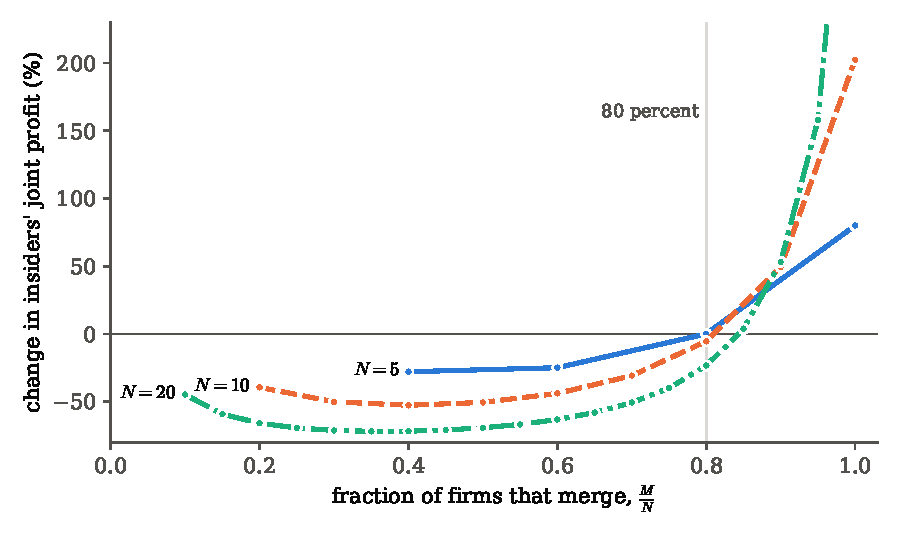
\includegraphics[width=0.8\textwidth]{figures/ch11/ssr_paradox.pdf}
\caption{The merger paradox. Percentage change in the joint profit of $M$ merging firms in a linear Cournot
market with $N$ symmetric firms and no cost savings, $100\big[\frac{(N + 1)^2}{M(N - M + 2)^2} - 1\big]$, against
$\frac{M}{N}$. Points above zero are profitable mergers. Curves are clipped at 230 percent.}
\label{fig:11-ssr}
\end{figure}

The reason is the response of the outsiders. In Cournot competition, quantities are strategic substitutes. When
the merged firm cuts its output, the outsiders expand theirs and capture much of the benefit of the higher price.
Moreover, a merger in this model is equivalent to $M - 1$ firms shutting down. The merged firm is no larger and no
more efficient than any other firm, so it ends up with a share of only $\frac{1}{N - M + 1}$
\citep[p.~4]{FarrellShapiro1988}. The paradox is that we observe many horizontal mergers.

Three features of the model drive the result, and relaxing any of them can overturn it. First, the merging firms
bring no assets. \citet{PerryPorter1985} let each firm own capital that lowers its marginal cost, so the merged
firm has the combined capital and is larger than its rivals. Mergers can then be profitable, and
\cref{sec:11-fs} develops this idea in general. Second, the model has no investment. \citet[Remark
3]{Pesendorfer2003} considers firms that hold capacity, with linear demand $P = a - bQ$, constant marginal cost
$c$, a linear cost $r$ per unit of new capacity, and initial capacities at Cournot levels. He also normalizes the
discount and depreciation factors. He shows that a merger
without cost savings is profitable whenever $n + 1 > \frac{a - c}{r}$. Building capacity is costly while scrapping
it is not, and this asymmetry favors the merged firm. The Salant-Switzer-Reynolds result is the limit as $r \to 0$
\citep[p.~7, n.~6]{Pesendorfer2003}. \Cref{sec:11-beyond} returns to this model. Third, quantities are strategic
substitutes. With price competition and differentiated products, rivals raise their prices after a merger, and
the merger is profitable (\cref{sec:11-upp}).

\subsection{Farrell and Shapiro (1990): mergers as transfers of capital}\label{sec:11-fs}

\casehead{The question}
\citet{FarrellShapiro1990} ask when a horizontal merger raises the price, when it raises welfare, and what a
regulator can infer from the fact that the merging firms want to merge. Their answer rests on three ideas. A merger
is a transfer of industry-specific capital from one firm to another. The welfare effect of a merger can be split
into the change in the merging firms' profits, which they internalize, and an \emph{external effect} on consumers
and rivals. The external effect depends only on observable market data, while the private effect may include
synergies that only the firms know. A regulator should therefore approve any merger that is proposed and has a
positive external effect, because private profitability then guarantees a welfare gain. We follow the 1988
working-paper version \citep{FarrellShapiro1988}, whose numbering of equations and propositions differs from the
published article. The result on the cost savings needed to lower the price belongs to the published article
\citep{FarrellShapiro1990} and is not in the working paper. We state it as \citet[pp.~216--217 and
229]{AskerNocke2021} report it, and we prove it in full.

\subsubsection{The model}

There are $N$ firms producing a homogeneous good, and their number is fixed by barriers to entry. A competitive
fringe can be absorbed into the demand curve, which is then a residual demand. We write $q_i$ for firm $i$'s
output, $Q = \sum_i q_i$ for industry output, $P(Q)$ for inverse demand and $s_i = \frac{q_i}{Q}$ for market
shares (Farrell and Shapiro write $x_i$, $X$ and $p(X)$).

\begin{assumption}[Cournot oligopoly with capital]\label{ass:11-fs}
\leavevmode
\begin{enumerate}[label=(\roman*)]
  \item Inverse demand $P(Q)$ is twice differentiable with $P'(Q) < 0$.
  \item Firm $i$ owns capital $k_i$ and has a twice differentiable cost function $C^i(q_i, k_i)$. More capital
  lowers marginal cost, $C^i_{qk} < 0$, where subscripts denote partial derivatives.
  \item Given the capital vector $k = (k_1, \dots, k_N)$, firms choose outputs simultaneously (Cournot). The
  equilibrium is unique and interior.
  \item Reaction functions slope down and the equilibrium is stable. Formally, at the equilibrium,
  $P' + q_i P'' < 0$ and $C^i_{qq} - P' > 0$ for every firm.
\end{enumerate}
\end{assumption}

Firms may have different technologies, and $C^i$ may then embody firm-specific assets that cannot be transferred.
Capital is industry specific and fixed in the short run, while outputs adjust quickly. Firm $i$ maximizes
$\pi_i = P(Q)\,q_i - C^i(q_i, k_i)$, with first-order condition
\begin{equation}\label{eq:11-fs-foc}
P(Q) + q_i P'(Q) - C^i_q(q_i, k_i) = 0, \qquad i = 1, \dots, N.
\end{equation}
The condition implies $P - C^i_q = -q_i P'$, so each firm's margin over marginal cost is proportional to its
output. Comparing two firms, $q_i > q_j$ if and only if $C^i_q < C^j_q$. In a Cournot equilibrium, \emph{larger
firms have lower marginal costs}. Whenever firms produce different quantities, marginal costs differ, so total
cost is not minimized for the industry's output. Shifting output toward large firms would lower it.

Welfare is consumers' gross benefit minus production costs,
\begin{equation*}
W = \int_0^Q P(z)\,\dd z - \sum_{i=1}^{N} C^i(q_i, k_i).
\end{equation*}

\subsubsection{Profit and welfare effects of a change in capital}

Consider a small change $\dd k = (\dd k_1, \dots, \dd k_N)$ in the allocation of capital, and the induced changes
$\dd q_i$ in outputs. Differentiating $\pi_i$,
\begin{equation}\label{eq:11-fs-dpi}
\dd\pi_i = (P - C^i_q)\,\dd q_i + q_i P'\,\dd Q - C^i_k\,\dd k_i .
\end{equation}
A firm gains from extra output in proportion to its margin, gains from a price increase in proportion to its
output, and saves costs through its own capital. Differentiating $W$ and using $\frac{\dd}{\dd Q}\int_0^Q P = P$,
\begin{equation}\label{eq:11-fs-dw}
\dd W = \sum_{i=1}^{N} (P - C^i_q)\,\dd q_i - \sum_{i=1}^{N} C^i_k\,\dd k_i .
\end{equation}
The first sum values each change in output at the gap between price and marginal cost. The second is the direct
effect of capital on costs at given outputs. Equations \eqref{eq:11-fs-dpi} and \eqref{eq:11-fs-dw} hold for any
theory of oligopoly. Under Cournot competition, $P - C^i_q = -q_i P'$, and \eqref{eq:11-fs-dw} becomes
\begin{equation}\label{eq:11-fs-dw-cournot}
\dd W = -P'\sum_{i=1}^{N} q_i\,\dd q_i - \sum_{i=1}^{N} C^i_k\,\dd k_i .
\end{equation}

\begin{lemma}[Welfare and the Herfindahl index]\label{lem:11-fs-hhi}
Under \cref{ass:11-fs},
\begin{equation}\label{eq:11-fs-dw-hhi}
\dd W = -P'\Big(\HHI\,Q\,\dd Q + \frac{1}{2}Q^2\,\dd\HHI\Big) - \sum_{i=1}^{N} C^i_k\,\dd k_i .
\end{equation}
\end{lemma}

\begin{proof}
Since $\HHI = \sum_i \big(\frac{q_i}{Q}\big)^2$, we have $Q^2\HHI = \sum_i q_i^2$. Differentiating both sides,
\begin{equation*}
2\sum_i q_i\,\dd q_i = \dd\big(Q^2\HHI\big) = 2\HHI\,Q\,\dd Q + Q^2\,\dd\HHI .
\end{equation*}
Dividing by two and substituting into \eqref{eq:11-fs-dw-cournot} gives \eqref{eq:11-fs-dw-hhi}.
\end{proof}

\Cref{lem:11-fs-hhi} splits a welfare change into three parts: a change in industry output, a change in its
distribution, and the direct effect on costs. More output raises welfare because price exceeds marginal cost.
More surprisingly, for a given change in output, a larger increase in the Herfindahl index raises welfare more,
since $-P' > 0$. Large firms have the lowest marginal costs, so shifting output toward them saves resources. Any
analysis that treats increases in concentration as bad per se is therefore misleading under Cournot competition
\citep[p.~8]{FarrellShapiro1988}.

\subsubsection{Comparative statics}

\begin{lemma}[Output responses]\label{lem:11-fs-statics}
Under \cref{ass:11-fs}, define for each firm
\begin{equation}\label{eq:11-fs-lambda}
\lambda_i = \frac{-P' - q_i P''}{C^i_{qq} - P'} > 0,
\qquad
\chi_i = \frac{-C^i_{qk}}{C^i_{qq} - P'} > 0,
\qquad
\Lambda = \sum_{i=1}^{N}\lambda_i .
\end{equation}
A small change $\dd k$ changes outputs by
\begin{equation}\label{eq:11-fs-dq}
\dd q_i = -\lambda_i\,\dd Q + \chi_i\,\dd k_i,
\qquad
\dd Q = \frac{1}{1 + \Lambda}\sum_{i=1}^{N}\chi_i\,\dd k_i .
\end{equation}
\end{lemma}

\begin{proof}
Totally differentiate the first-order condition \eqref{eq:11-fs-foc}, holding the equilibrium:
\begin{equation*}
\big(P' + q_i P''\big)\,\dd Q + P'\,\dd q_i - C^i_{qq}\,\dd q_i - C^i_{qk}\,\dd k_i = 0 .
\end{equation*}
Collect the terms in $\dd q_i$:
\begin{equation*}
\big(C^i_{qq} - P'\big)\,\dd q_i = \big(P' + q_i P''\big)\,\dd Q - C^i_{qk}\,\dd k_i .
\end{equation*}
Dividing by $C^i_{qq} - P' > 0$ gives the first part of \eqref{eq:11-fs-dq}. Signs follow from part (iv) of
\cref{ass:11-fs} and from $C^i_{qk} < 0$. Summing over $i$,
\begin{equation*}
\dd Q = -\Lambda\,\dd Q + \sum_i \chi_i\,\dd k_i ,
\end{equation*}
and solving for $\dd Q$ gives the second part.
\end{proof}

The coefficient $\chi_i$ is the \emph{direct effect} of firm $i$'s capital on its output at a given industry
output (Farrell and Shapiro call it $\delta_i$). The coefficient $\lambda_i$ measures how firm $i$ responds to a
change in industry output, and hence to the price. A firm whose capital does not change adjusts its output by
$\dd q_i = -\lambda_i\,\dd Q$. Its response to the combined output of the others, $Q_{-i}$, follows from
$\dd Q = \dd q_i + \dd Q_{-i}$ and is $\frac{\dd q_i}{\dd Q_{-i}} = -\frac{\lambda_i}{1 + \lambda_i}$. Two special
cases recur. With constant marginal cost, $C^i_{qq} = 0$ and
\begin{equation}\label{eq:11-fs-lambda-const}
\lambda_i = \frac{-P' - q_i P''}{-P'} = 1 + \frac{q_i P''}{P'} = 1 - s_i\,\mathcal{E},
\qquad
\mathcal{E} = -\frac{Q P''(Q)}{P'(Q)},
\end{equation}
where $\mathcal{E}$ is the elasticity of the slope of inverse demand (Farrell and Shapiro write $E$). With linear
demand $P = a - Q$ and the cost function $C(q, k) = \frac{q^2}{2k}$, we have $C_{qq} = \frac{1}{k}$ and
$P' = -1$, so $\lambda_i = \frac{1}{1 + \frac{1}{k_i}} = \frac{k_i}{1 + k_i}$.

\begin{example}[Two technologies]\label{ex:11-fs-tech}
\emph{Physical capital.} Let $P(Q) = a - Q$ and $C(q, k) = \frac{q^2}{2k}$ for all firms. This technology has
constant returns to scale and corresponds to the production function $q = \sqrt{kv}$ with a variable input $v$.
Firm $i$'s first-order condition is $a - Q - q_i - \frac{q_i}{k_i} = 0$. Define the \emph{adjusted capital}
$\tilde k_i = \frac{k_i}{1 + k_i}$. The condition becomes
\begin{equation*}
q_i\Big(1 + \frac{1}{k_i}\Big) = a - Q
\quad\Longrightarrow\quad
q_i = (a - Q)\,\tilde k_i = P\,\tilde k_i .
\end{equation*}
Summing over firms, $Q = (a - Q)\tilde K$ with $\tilde K = \sum_i \tilde k_i$, so
\begin{equation*}
Q = \frac{a\tilde K}{1 + \tilde K}, \qquad P = \frac{a}{1 + \tilde K}, \qquad
C^i_q = \frac{q_i}{k_i} = \frac{P}{1 + k_i} .
\end{equation*}
Firms with more capital produce more and have lower marginal costs. Here $\lambda_i = \tilde k_i = \frac{q_i}{P}$,
and the direct effect is
\begin{equation*}
\chi_i = \frac{\frac{q_i}{k_i^2}}{\frac{1}{k_i} + 1} = \frac{q_i}{k_i(1 + k_i)} = \frac{P}{(1 + k_i)^2} .
\end{equation*}
\emph{Know-how.} Let unit cost depend on capital but not on output, $C(q, k) = q\,\phi(k)$ with $\phi' < 0$. This
fits patents, know-how and managerial talent, which can be applied to any scale of output. The first-order
conditions are $P + q_i P' = \phi(k_i)$, and summing them gives
\begin{equation}\label{eq:11-fs-knowhow}
N P(Q) + Q P'(Q) = \sum_{i=1}^{N}\phi(k_i),
\end{equation}
so industry output depends on capital only through the sum of marginal costs.
\end{example}

\subsubsection{Investment by one firm}

Before turning to mergers, consider investment, $\dd k = (\dd k_1, 0, \dots, 0)$. By \cref{lem:11-fs-statics},
\begin{equation*}
\frac{\dd Q}{\dd k_1} = \frac{\chi_1}{1 + \Lambda}, \qquad
\frac{\dd q_i}{\dd k_1} = -\frac{\lambda_i\chi_1}{1 + \Lambda}\ (i \ne 1), \qquad
\frac{\dd q_1}{\dd k_1} = \chi_1\Big(1 - \frac{\lambda_1}{1 + \Lambda}\Big).
\end{equation*}
The investing firm expands, its rivals contract, and industry output rises. Subtracting \eqref{eq:11-fs-dw} from
\eqref{eq:11-fs-dpi} for $i = 1$, the private and social returns differ by
\begin{equation}\label{eq:11-fs-invest-wedge0}
\dd\pi_1 - \dd W = q_1 P'\,\dd Q - \sum_{i \ne 1}(P - C^i_q)\,\dd q_i .
\end{equation}
The first term is a private loss that is a transfer to consumers: the investor's price falls on its own sales. The
second is a social cost the investor ignores: rivals, whose price exceeds marginal cost, cut their output. Using
$P - C^i_q = -q_i P'$ and $\dd q_i = -\lambda_i\,\dd Q$ for $i \ne 1$,
\begin{equation}\label{eq:11-fs-invest-wedge}
\frac{\dd\pi_1}{\dd k_1} - \frac{\dd W}{\dd k_1}
= -P'\,\frac{\dd Q}{\dd k_1}\Big(\sum_{i \ne 1}\lambda_i q_i - q_1\Big).
\end{equation}

\begin{proposition}[Investment incentives]\label{prop:11-fs-invest}
Under \cref{ass:11-fs}, firm 1 has an excessive incentive to invest, $\frac{\dd\pi_1}{\dd k_1} >
\frac{\dd W}{\dd k_1}$, if and only if
\begin{equation}\label{eq:11-fs-invest}
s_1 < \sum_{i \ne 1}\lambda_i s_i .
\end{equation}
With linear demand and the costs $\frac{q^2}{2k}$, the condition is $s_1 < \frac{1}{\varepsilon}\sum_{i \ne 1}s_i^2$,
where $\varepsilon = -\frac{P}{QP'}$. With constant marginal costs, it is
$s_1 < \frac{1}{2} - \frac{\mathcal{E}}{2}\sum_{i \ne 1}s_i^2$.
\end{proposition}

\begin{proof}
In \eqref{eq:11-fs-invest-wedge}, $-P' > 0$ and $\frac{\dd Q}{\dd k_1} > 0$, so the wedge is positive if and only
if $\sum_{i \ne 1}\lambda_i q_i > q_1$. Dividing by $Q$ gives \eqref{eq:11-fs-invest}. In the quadratic case,
$\lambda_i = \frac{q_i}{P}$, so $\sum_{i \ne 1}\lambda_i s_i = \frac{Q}{P}\sum_{i \ne 1}s_i^2$, and
$\frac{Q}{P} = \frac{1}{\varepsilon}$ because $P' = -1$. With constant marginal costs,
$\sum_{i \ne 1}(1 - s_i\mathcal{E})s_i = 1 - s_1 - \mathcal{E}\sum_{i \ne 1}s_i^2$, and the inequality
$s_1 < 1 - s_1 - \mathcal{E}\sum_{i \ne 1}s_i^2$ rearranges to the stated form.
\end{proof}

Small firms invest too much. Their investment lowers the price and helps consumers, but it steals valuable
business from larger rivals with high margins, and the second effect dominates \citep[pp.~10--11]{FarrellShapiro1988}.
If $\lambda_i$ rises with firm size, as in the quadratic case, large efficient firms invest too little.

\subsubsection{Small capital transfers and the price}

A merger moves capital from one firm to another. Consider a small transfer from firm 2 to firm 1,
$\dd k_1 = \dd k = -\dd k_2 > 0$, with $k_1 > k_2$, so that the transfer increases the concentration of capital.
A complete merger of the two firms is the accumulation of such transfers, from $(k_1, k_2)$ to $(k_1 + k_2, 0)$.
Divestitures are the reverse.

\begin{proposition}[Price effect of a transfer]\label{prop:11-fs-price}
Under \cref{ass:11-fs}, a small transfer of capital from firm 2 to firm 1 changes industry output by
\begin{equation}\label{eq:11-fs-dqdk}
\frac{\dd Q}{\dd k} = \frac{\chi_1 - \chi_2}{1 + \Lambda}.
\end{equation}
It reduces output and raises the price if and only if $\chi_1 < \chi_2$, that is, if and only if the direct
output effect of capital is smaller at the acquiring firm.
\end{proposition}

\begin{proof}
Substitute $\dd k_1 = \dd k$, $\dd k_2 = -\dd k$ and $\dd k_i = 0$ for $i \ge 3$ into \eqref{eq:11-fs-dq}. Since
$1 + \Lambda > 0$, the sign of $\dd Q$ is the sign of $\chi_1 - \chi_2$.
\end{proof}

In the physical-capital example, $\chi_i = \frac{P}{(1 + k_i)^2}$ falls with $k_i$, so every
concentration-increasing transfer raises the price. The same follows from the closed form $P = \frac{a}{1 + \tilde
K}$. Adjusted capital $\tilde k(k) = \frac{k}{1 + k}$ is strictly concave with $\tilde k(0) = 0$, so moving capital
from the smaller to the larger firm lowers $\tilde k_1 + \tilde k_2$, and a complete merger gives
$\tilde k(k_1 + k_2) < \tilde k(k_1) + \tilde k(k_2)$. In the know-how example, \eqref{eq:11-fs-knowhow} shows
that output falls if and only if the transfer raises $\sum_i\phi(k_i)$, and the transfer changes this sum by
$\big(\phi'(k_1) - \phi'(k_2)\big)\dd k$. With $k_1 > k_2$, the price rises if and only if $\phi'' > 0$. A merger of
know-how raises the price when units of know-how are substitutes, which lower unit cost at a diminishing rate. It
lowers the price when they are complements.

\Cref{prop:11-fs-price} needs the $\chi_i$, which are hard to measure. A condition on the technology alone is more
useful.

\begin{proposition}[A sufficient condition, \citealp{FarrellShapiro1988}]\label{prop:11-fs-convex}
Suppose that, in addition to \cref{ass:11-fs}, all firms share the cost function $C(q, k)$ and the marginal cost
$C_q$ is jointly convex in $(q, k)$. Then every concentration-increasing transfer, small or large, weakly reduces
output and weakly raises the price, as long as the selling firm remains active. The effects are strict when the Hessian
of $C_q$ is positive definite.
\end{proposition}

\begin{proof}
Fix industry output $Q$, and let $\tilde q(Q, k)$ be the output of a firm with capital $k$ that satisfies the
first-order condition, $P(Q) + \tilde q P'(Q) = C_q(\tilde q, k)$. Because the technology is common, firm $i$'s output in
equilibrium is $\tilde q(Q, k_i)$ and its direct effect is $\chi_i = \tilde q_k(Q, k_i)$. To see this, differentiate the
condition in $k$ at fixed $Q$:
\begin{equation*}
P'\,\tilde q_k = C_{qq}\,\tilde q_k + C_{qk}
\quad\Longrightarrow\quad
\tilde q_k = \frac{-C_{qk}}{C_{qq} - P'} = \chi .
\end{equation*}
Differentiating once more in $k$,
\begin{equation*}
P'\,\tilde q_{kk} = C_{qqq}\,\tilde q_k^2 + 2C_{qqk}\,\tilde q_k + C_{qkk} + C_{qq}\,\tilde q_{kk},
\end{equation*}
so
\begin{equation*}
\tilde q_{kk} = -\frac{C_{qqq}\,\tilde q_k^2 + 2C_{qqk}\,\tilde q_k + C_{qkk}}{C_{qq} - P'} .
\end{equation*}
The numerator is $\gamma^\top H\gamma$ with $\gamma = (\tilde q_k, 1)^\top$ and $H$ the Hessian of $C_q$. Joint
convexity makes it nonnegative, so $\tilde q_{kk} \le 0$ and $\chi = \tilde q_k$ is nonincreasing in $k$ across firms.
Hence $k_1 > k_2$ implies $\chi_1 \le \chi_2$, and \cref{prop:11-fs-price} applies. A positive definite Hessian
makes the numerator positive, because $\gamma \ne 0$, and then $\chi_1 < \chi_2$. A large transfer is a sequence of small transfers, each from the smaller to the larger firm,
so output falls along the whole path.
\end{proof}

Farrell and Shapiro add that the condition is sufficient but not necessary. The physical-capital technology
violates it, since its marginal cost $\frac{q}{k}$ is not jointly convex, yet every merger raises the price there.
The know-how technology satisfies it exactly when $\phi'' \ge 0$, since $C_q = \phi(k)$. Its Hessian is
singular, yet the numerator in the proof equals $\phi''(k)$, so the price rises strictly when $\phi'' > 0$. Under the conditions of
\cref{prop:11-fs-price,prop:11-fs-convex}, a merger harms consumers. Because rivals' profits rise exactly when the
price rises, the same conditions tell us when rivals gain \citep[p.~15]{FarrellShapiro1988}.

\subsubsection{Discrete mergers and the synergies needed to lower the price}

A merger can also reorganize production or create synergies that a reallocation of existing capital cannot
capture. To study such mergers, we replace capital by constant marginal costs. Firm $i$ has marginal cost $c_i$.
Firms 1 and 2 merge, and the merged firm has marginal cost $c_M$, which summarizes its post-merger technology. A
merger with no synergies can at best produce everything at the lower of the two costs, $c_M = \min\{c_1, c_2\}$.
We write $P^0 = P(Q^0)$ for the pre-merger price.

\begin{proposition}[Synergies needed to lower the price, \citealp{FarrellShapiro1990}]\label{prop:11-synergy}
Suppose firms have constant marginal costs, $P'(Q) + qP''(Q) < 0$ for all $0 \le q \le Q$, and all firms are active
before and after the merger. The merger of firms 1 and 2 lowers the equilibrium price if and only if
\begin{equation}\label{eq:11-synergy}
c_M < \hat c \equiv c_1 + c_2 - P^0,
\quad\text{equivalently}\quad
P^0 - c_M > (P^0 - c_1) + (P^0 - c_2).
\end{equation}
It leaves the price unchanged if $c_M = \hat c$ and raises it if $c_M > \hat c$.
\end{proposition}

\begin{proof}
Summing the first-order conditions $P + q_i P' = c_i$ over the $n$ active firms gives the aggregate condition
\begin{equation*}
\Gamma_n(Q) \equiv nP(Q) + QP'(Q) = \sum_{i \text{ active}} c_i .
\end{equation*}
Its slope is $\Gamma_n'(Q) = P' + \sum_{i}\big(P' + q_i P''\big) < 0$, so $\Gamma_n$ is strictly decreasing and
the equilibrium output is the unique solution. Only the number of firms and the sum of their marginal costs
matter for $Q$. Before the merger,
\begin{equation*}
N P^0 + Q^0 P'(Q^0) = c_1 + c_2 + \sum_{i \ge 3} c_i .
\end{equation*}
After the merger there are $N - 1$ firms, and the post-merger output $Q^1$ solves
$\Gamma_{N-1}(Q^1) = c_M + \sum_{i \ge 3}c_i$. Evaluate $\Gamma_{N-1}$ at the pre-merger output and use the
pre-merger condition:
\begin{equation*}
\Gamma_{N-1}(Q^0) = N P^0 + Q^0 P'(Q^0) - P^0 = c_1 + c_2 - P^0 + \sum_{i \ge 3}c_i .
\end{equation*}
Since $\Gamma_{N-1}$ is decreasing, $Q^1 > Q^0$ if and only if
$\Gamma_{N-1}(Q^1) < \Gamma_{N-1}(Q^0)$, that is, if and only if
\begin{equation*}
c_M + \sum_{i \ge 3}c_i < c_1 + c_2 - P^0 + \sum_{i \ge 3}c_i
\quad\Longleftrightarrow\quad
c_M < c_1 + c_2 - P^0 .
\end{equation*}
A higher output means a lower price. The cases of equality and of the reverse inequality follow the same way.
\end{proof}

\begin{corollary}[No synergies, higher price]\label{prop:11-nosynergy}
Under the conditions of \cref{prop:11-synergy}, the price-neutral cost satisfies $\hat c < \min\{c_1, c_2\}$.
Any merger with $c_M \ge \min\{c_1, c_2\}$, including every merger that only rationalizes production, raises the
price.
\end{corollary}

\begin{proof}
Firm 2 is active before the merger, so $P^0 - c_2 = -q_2 P'(Q^0) > 0$. Hence
$\hat c = c_1 - (P^0 - c_2) < c_1$. By the same argument with the roles reversed, $\hat c < c_2$. If
$c_M \ge \min\{c_1, c_2\}$, then $c_M > \hat c$, and \cref{prop:11-synergy} applies.
\end{proof}

The required synergy is large. Let firm 1 be the more efficient partner. The merged firm's cost must fall below
$c_1$ by firm 2's entire margin, $c_1 - \hat c = P^0 - c_2$. As a fraction of the price, the reduction equals firm
2's Lerner index, $\frac{c_1 - \hat c}{P^0} = \frac{s_2}{\varepsilon}$. As a fraction of firm 1's cost it is
$\frac{L_2}{1 - L_1}$, where $L_i = \frac{P^0 - c_i}{P^0}$. Two firms with 20 percent shares each, facing a market
elasticity of one, have $L_1 = L_2 = 0.2$. For their merger not to raise the price, marginal cost must fall by
$\frac{0.2}{0.8} = 25$ percent.

The required reduction can also be written with the naive change in concentration. Let $s_I = s_1 + s_2$ and let
$\bar c = \frac{s_1 c_1 + s_2 c_2}{s_I}$ be the partners' share-weighted marginal cost. The first-order conditions
give $P^0 - c_i = \frac{s_i P^0}{\varepsilon}$, so
\begin{align*}
P^0 - \bar c &= \frac{s_1(P^0 - c_1) + s_2(P^0 - c_2)}{s_I} = \frac{s_1^2 + s_2^2}{s_I}\cdot\frac{P^0}{\varepsilon},\\
P^0 - \hat c &= (P^0 - c_1) + (P^0 - c_2) = s_I\,\frac{P^0}{\varepsilon}.
\end{align*}
Subtracting the first line from the second,
\begin{equation}\label{eq:11-required-dhhi}
\frac{\bar c - \hat c}{P^0} = \frac{1}{\varepsilon}\Big(s_I - \frac{s_1^2 + s_2^2}{s_I}\Big)
= \frac{(s_1 + s_2)^2 - s_1^2 - s_2^2}{\varepsilon\, s_I} = \frac{2 s_1 s_2}{\varepsilon\, s_I} .
\end{equation}
The numerator is the naive $\Delta\HHI$ of \eqref{eq:11-dhhi}. The outsiders' shares do not enter, so for given
shares of the merging firms the required efficiency does not depend on the level of the index. This parallels the
finding of \citet{NockeWhinston2020}, reported in \cref{sec:11-hhi}, that required efficiencies track the change in
concentration and not its level. In the example above,
$\frac{2 \times 0.2 \times 0.2}{0.4} = 0.2$ of the price, which is 25 percent of $\bar c = 0.8 P^0$.

\Cref{prop:11-synergy} is the condition that \citet[Lemma 1 and eq.~(5)]{NockeWhinston2013} use to define a
\emph{CS-neutral merger}, one that leaves consumer surplus unchanged. In their notation, with acquirer 0 and
target $k$, the condition is $\bar c_k = c_k - \big[P(Q^0) - c_0\big]$, the same as \eqref{eq:11-synergy}. They also
note that such a merger is profitable. The argument is short.

\begin{corollary}[A price-neutral merger is profitable]\label{cor:11-neutral-profit}
Under the conditions of \cref{prop:11-synergy}, let $c_M = \hat c$. The merger leaves the price and every
outsider's output unchanged and gives the merged firm the output $q_1 + q_2$. It raises the joint profit of the
merging firms by $(P^0 - c_1)q_2 + (P^0 - c_2)q_1 > 0$.
\end{corollary}

\begin{proof}
With $c_M = \hat c$, \cref{prop:11-synergy} gives $Q^1 = Q^0$, so the price and its slope are unchanged. Each
outsider's first-order condition $P + q_i P' = c_i$ then gives the same $q_i$. The merged firm produces the rest,
$Q^0 - \sum_{i \ge 3}q_i = q_1 + q_2$. Its profit is
\begin{align*}
(P^0 - \hat c)(q_1 + q_2)
&= \big[(P^0 - c_1) + (P^0 - c_2)\big](q_1 + q_2) \\
&= \underbrace{(P^0 - c_1)q_1 + (P^0 - c_2)q_2}_{\pi_1 + \pi_2} + (P^0 - c_1)q_2 + (P^0 - c_2)q_1 .
\end{align*}
Both extra terms are positive because both firms were active.
\end{proof}

\Cref{fig:11-synergy} illustrates these results. Demand is $P = 10 - Q$ and three firms have costs
$(c_1, c_2, c_3) = (2, 3, 3)$, so $P^0 = 4.5$ and outputs are $(2.5, 1.5, 1.5)$. If firms 1 and 2 merge, the
post-merger price is $\frac{13 + c_M}{3}$. The price-neutral cost is $\hat c = 2 + 3 - 4.5 = 0.5$, well below
$c_1 = 2$. Rationalization alone, $c_M = 2$, raises the price to 5. This merger is still profitable, because the
merged firm earns 9 against the 8.5 the two firms earned before. It lowers total surplus by 0.375, as consumers
lose 2.625 while the outsider gains 1.75. Every cost between 0.5 and about 2.13 makes the merger both profitable
and price-increasing. Total surplus rises only for costs below about 1.91.

\begin{figure}[htbp]
\centering
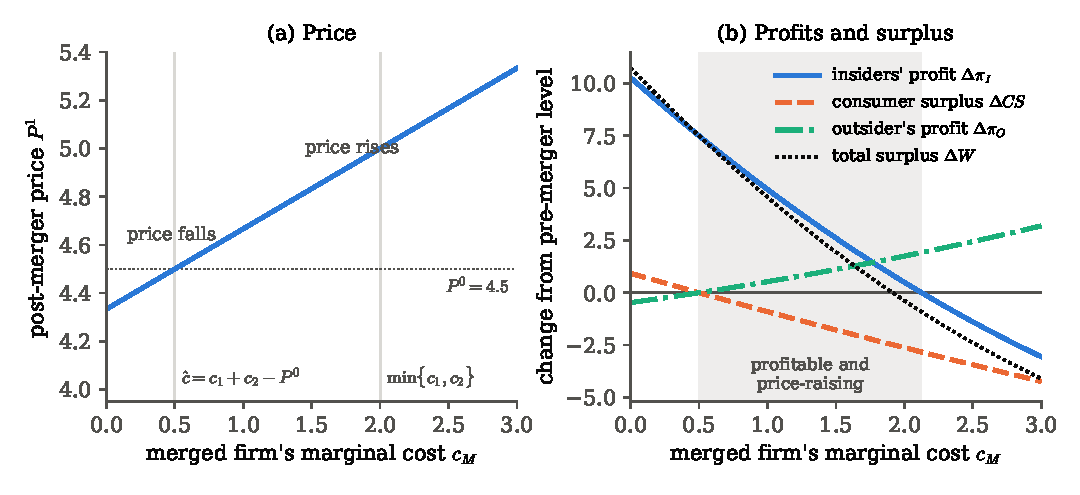
\includegraphics[width=\textwidth]{figures/ch11/cournot_synergy.pdf}
\caption{A Cournot merger with constant marginal costs. Demand $P = 10 - Q$, costs $(c_1, c_2, c_3) = (2, 3, 3)$,
and firms 1 and 2 merge with marginal cost $c_M$. Panel (a) shows the post-merger price, with the price-neutral cost
$\hat c = 0.5$ and the rationalization cost $\min\{c_1, c_2\} = 2$. Panel (b) shows the changes in the insiders'
joint profit, consumer surplus, the outsider's profit and total surplus. The shaded band, $0.5 < c_M < 2.13$, contains
the mergers that are profitable and raise the price. Total surplus falls for $c_M > 1.91$.}
\label{fig:11-synergy}
\end{figure}

\subsubsection{General costs, many partners and aggregate surplus}

\Cref{prop:11-synergy} assumes constant marginal costs and two partners. \citet[p.~229, eq.~(6)]{AskerNocke2021}
state the condition of \citet{FarrellShapiro1990} for any cost functions and any number of partners. We hold capital
fixed and write $C_i(q_i)$ for firm $i$'s cost function. A set $\mathcal{M}$ of at least two firms merges into a firm
with cost function $C_{\mathcal{M}}(q)$, and $q_{\mathcal{M}}^0 = \sum_{i \in \mathcal{M}} q_i^0$ is the partners'
combined pre-merger output.

\begin{proposition}[The synergy condition with general costs, \citealp{FarrellShapiro1990}]\label{prop:11-synergy-gen}
Let \cref{ass:11-fs} hold with capital fixed, let $C''_{\mathcal{M}} - P' > 0$, and let all firms be active before
and after the merger. The merger weakly raises industry output, and so does not lower consumer surplus, if and only
if
\begin{equation}\label{eq:11-an6}
P(Q^0) - C'_{\mathcal{M}}\big(q_{\mathcal{M}}^0\big) \;\ge\; \sum_{i \in \mathcal{M}}\big[P(Q^0) - C'_i(q_i^0)\big].
\end{equation}
It weakly lowers industry output if and only if the reverse weak inequality holds.
\end{proposition}

\begin{proof}
For a firm with cost function $C$, define its \emph{fitting-in output} $r(Q)$ as the solution in $q$ of $P(Q) +
qP'(Q) = C'(q)$. It is the output at which the firm's first-order condition holds when industry output is $Q$. The
left side minus the right side falls in $q$ at rate $P' - C'' < 0$, so $r(Q)$ is unique. Differentiating the
condition in $Q$,
\begin{equation*}
P' + r'P' + rP'' = C''r'
\quad\Longrightarrow\quad
r'(Q) = \frac{P' + rP''}{C'' - P'} = -\lambda ,
\end{equation*}
with $\lambda > 0$ the response coefficient of \cref{lem:11-fs-statics}. An equilibrium is an industry output at
which the fitting-in outputs add up to $Q$. After the merger, let
\begin{equation*}
\Phi(Q) = \sum_{i \notin \mathcal{M}} r_i(Q) + r_{\mathcal{M}}(Q) - Q .
\end{equation*}
It is strictly decreasing, with slope $-\sum_{i \notin \mathcal{M}}\lambda_i - \lambda_{\mathcal{M}} - 1 < 0$, so
the post-merger output $Q^1$ is its unique zero, and $Q^1 \ge Q^0$ if and only if $\Phi(Q^0) \ge 0$. At $Q^0$ each
outsider's fitting-in output is its pre-merger output, $r_i(Q^0) = q_i^0$. Hence
\begin{equation*}
\Phi(Q^0) = \sum_{i \notin \mathcal{M}} q_i^0 + r_{\mathcal{M}}(Q^0) - Q^0 = r_{\mathcal{M}}(Q^0) - q_{\mathcal{M}}^0 .
\end{equation*}
The merged firm's marginal profit at fixed $Q^0$, $P(Q^0) + qP'(Q^0) - C'_{\mathcal{M}}(q)$, falls in $q$ and is
zero at $r_{\mathcal{M}}(Q^0)$. So $r_{\mathcal{M}}(Q^0) \ge q_{\mathcal{M}}^0$ if and only if the marginal profit
is nonnegative at $q_{\mathcal{M}}^0$:
\begin{equation*}
P(Q^0) + q_{\mathcal{M}}^0P'(Q^0) - C'_{\mathcal{M}}\big(q_{\mathcal{M}}^0\big) \ge 0 .
\end{equation*}
The partners' pre-merger first-order conditions give $q_i^0P'(Q^0) = -\big[P(Q^0) - C'_i(q_i^0)\big]$. Summing over
$i \in \mathcal{M}$,
\begin{equation*}
q_{\mathcal{M}}^0P'(Q^0) = -\sum_{i \in \mathcal{M}}\big[P(Q^0) - C'_i(q_i^0)\big] .
\end{equation*}
Substituting into the marginal profit gives \eqref{eq:11-an6}. The reverse case follows from the same steps with
the inequalities reversed.
\end{proof}

With constant marginal costs and two partners, \eqref{eq:11-an6} is \eqref{eq:11-synergy}. Every term on the right of
\eqref{eq:11-an6} is positive, because each partner was active. The right side therefore exceeds each single term
$P(Q^0) - C'_j(q_j^0)$. The condition thus requires the merged firm's marginal cost at the combined output to lie
below the pre-merger marginal cost of every partner, $C'_{\mathcal{M}}(q_{\mathcal{M}}^0) < \min_{i \in
\mathcal{M}}C'_i(q_i^0)$ \citep[p.~229]{AskerNocke2021}.

A merger can raise productive efficiency even without synergies, in the sense of \citet{FarrellShapiro1990}. Say
the merger creates \emph{no synergies} when the merged firm can do no better than allocate output among the
partners' existing technologies,
\begin{equation}\label{eq:11-nosynergy-cost}
C_{\mathcal{M}}(q) = \min\Big\{\sum_{i \in \mathcal{M}}C_i(q_i) : \sum_{i \in \mathcal{M}}q_i = q,\ q_i \ge 0\Big\}.
\end{equation}
By the pre-merger first-order conditions, $P - C'_i(q_i^0) = -q_i^0P'$, so the smaller partner has the higher
marginal cost. Shifting output from it to the larger partner lowers the cost of producing $q_{\mathcal{M}}^0$. The
next result shows that such output shifting is not enough.

\begin{corollary}[Rationalization is not enough]\label{cor:11-rationalize}
Under the conditions of \cref{prop:11-synergy-gen}, suppose every $C_i$ is convex and the merger creates no
synergies, as in \eqref{eq:11-nosynergy-cost}. Then the merger strictly lowers industry output and consumer surplus.
\end{corollary}

\begin{proof}
Let $(q_i^*)_{i \in \mathcal{M}}$ solve the problem in \eqref{eq:11-nosynergy-cost} at $q = q_{\mathcal{M}}^0$. By
the envelope theorem, $C'_{\mathcal{M}}(q_{\mathcal{M}}^0)$ equals the multiplier on the output constraint, which
equals $C'_i(q_i^*)$ for every partner with $q_i^* > 0$. The $q_i^*$ add up to $\sum_{i \in \mathcal{M}}q_i^0$, so
some partner $j$ has $q_j^* \ge q_j^0 > 0$. Convexity of $C_j$ gives
\begin{equation*}
C'_{\mathcal{M}}\big(q_{\mathcal{M}}^0\big) = C'_j(q_j^*) \ge C'_j(q_j^0) \ge \min_{i \in \mathcal{M}}C'_i(q_i^0) .
\end{equation*}
This violates the necessary condition stated after \cref{prop:11-synergy-gen}, so \eqref{eq:11-an6} fails, the
reverse strict inequality holds, and $Q^1 < Q^0$.
\end{proof}

The result extends to multiproduct firms that compete in prices under logit, nested logit or CES demand.
\citet{NockeSchutz2018,NockeSchutz2019} show that each firm can then be summarized by a single number, its
\emph{type}, which measures its contribution to consumer surplus if it priced at cost. Without synergies the merged
firm's type is the sum of the partners' types. A merger does not lower consumer surplus if and only if the merged
firm's type exceeds a cutoff above that sum, so it again requires synergies \citep[p.~229]{AskerNocke2021}.

\begin{figure}[htbp]
\centering
\begin{tikzpicture}[x=1.5cm, y=1.25cm, font=\small]
  \fill[gray!22] (0,4.25) -- (0,4.5) -- (5.5,4.5) -- (5.75,4.25) -- cycle;
  \fill[gray!60] (5.5,3.5) rectangle (5.75,4.25);
  \fill[pattern=north east lines, pattern color=black!65] (3.25,1) rectangle (3.5,2.5);
  \fill[pattern=north east lines, pattern color=black!65] (5.0,2.5) rectangle (5.5,3.5);
  \draw (3.25,1) rectangle (3.5,2.5);
  \draw (5.0,2.5) rectangle (5.5,3.5);
  \draw[->] (0,0) -- (7.4,0) node[below] {$Q$};
  \draw[->] (0,0) -- (0,5.6) node[left] {$p$};
  \draw[thick] (4.5,5.5) -- (7.2,2.8) node[right] {$P(Q)$};
  \draw (0,1) -- (6.9,1) node[right] {$c_1$};
  \draw (0,2.5) -- (6.9,2.5) node[right] {$c_2$};
  \draw (0,3.5) -- (6.9,3.5) node[right] {$c_3$};
  \draw[dashed] (0,4.25) -- (5.75,4.25);
  \draw[dashed] (0,4.5) -- (5.5,4.5);
  \node[left, font=\scriptsize] at (0,4.18) {$P^0$};
  \node[left, font=\scriptsize] at (0,4.6) {$P^1$};
  \foreach \x in {3.25,3.5,5.0,5.5,5.75} {\draw[dotted] (\x,0) -- (\x,4.5);}
  \node[below, font=\scriptsize] at (3.25,0) {$q_1^0$};
  \node[below, font=\scriptsize] at (3.5,-0.38) {$q_1^1$};
  \node[below, font=\scriptsize] at (5.0,0) {$q_1^0 + q_2^0$};
  \node[below, font=\scriptsize] at (5.5,-0.38) {$Q^1$};
  \node[below, font=\scriptsize] at (5.8,0) {$Q^0$};
\end{tikzpicture}
\caption{A Cournot merger without synergies, redrawn after \citet[Figure 6]{AskerNocke2021}. Demand is $P = 10 - Q$
and marginal costs are $c_1 = 1$, $c_2 = 2.5$ and $c_3 = 3.5$. Firms 2 and 3 merge and produce at $c_2$. The price
rises from $P^0 = 4.25$ to $P^1 = 4.5$, and output falls from $Q^0 = 5.75$ to $Q^1 = 5.5$. The light trapezoid is the
loss of consumer surplus (1.41). The dark rectangle is the margin lost on units that are no longer produced (0.19).
The hatched rectangles are cost savings, from output that moves to firm 1 (0.375) and from former firm-3 output now
produced at $c_2$ (0.5). Our computation.}
\label{fig:11-an-fig6}
\end{figure}

\Cref{fig:11-an-fig6} redraws the diagram that \citet[pp.~216--217]{AskerNocke2021} use to introduce merger analysis.
Firms 2 and 3 merge without synergies, so the merged firm produces at $c_2$. By \cref{prop:11-nosynergy} the price
rises. Firm 1 expands from $q_1^0 = 3.25$ to $q_1^1 = 3.5$, and the merged firm produces 2, less than the 2.5 that
firms 2 and 3 produced before. The welfare accounting has four pieces. Consumers lose the light trapezoid,
$(P^1 - P^0)Q^1 + \frac{1}{2}(P^1 - P^0)(Q^0 - Q^1) = 1.375 + 0.031$. The rectangle $(P^1 - P^0)Q^1$ is a transfer to
the firms, so only the triangle is a deadweight loss. The units between $Q^1$ and $Q^0$ were produced by firm 3 at
cost $c_3$, and their lost margin $(P^0 - c_3)(Q^0 - Q^1) = 0.1875$ is the dark rectangle. Production costs fall on
the remaining output, by $(c_2 - c_1)(q_1^1 - q_1^0) = 0.375$ and $(c_3 - c_2)\big(Q^1 - q_1^0 - q_2^0\big) = 0.5$.
Aggregate surplus therefore changes by
\begin{equation*}
\Delta W = -0.031 - 0.1875 + 0.375 + 0.5 = 0.656 > 0 .
\end{equation*}
Asker and Nocke leave the sign open for the case they draw, and they suggest that the reallocation gain may fall short
of the losses there (p.~216). With our numbers the reallocation gain dominates. The merger harms consumers, by 1.41, but raises aggregate surplus, because it moves production away from the least
efficient firm. It is also profitable, since the insiders gain 0.375. The price-neutral cost is $\hat c = c_2 + c_3 -
P^0 = 1.75$, so a merged firm with firm 1's cost of 1 would lower the price.

Two further results link consumer surplus, profit and aggregate surplus \citep[p.~230]{AskerNocke2021}. With
constant marginal costs, a merger that does not lower consumer surplus is profitable \citep{NockeWhinston2010}.
\Cref{cor:11-neutral-profit} shows this for the price-neutral merger, and a lower merged cost only raises the merged
firm's profit (\cref{lem:11-nw2}). A price-neutral merger leaves every outsider's output and profit unchanged, so it
raises aggregate surplus. The converse direction is less tidy. Aggregate surplus is not monotone in a firm's marginal
cost, so a given merger need not have a cutoff cost below which it raises aggregate surplus and above which it lowers
it. In the example of \cref{fig:11-synergy}, a cutoff does exist, near $c_M = 1.91$. Total surplus is still not
monotone. With the outsider's cost at 3, the derivative of total surplus in $c_M$ is
\begin{equation*}
\frac{\dd W}{\dd c_M} = (P - c_M)\frac{\dd q_M}{\dd c_M} + (P - 3)\frac{\dd q_3}{\dd c_M} - q_M
= -\frac{2}{3}q_M + \frac{1}{3}q_3 - q_M = \frac{q_3 - 5q_M}{3} .
\end{equation*}
It turns positive once the merged firm produces less than a fifth of the outsider's output, which happens for $c_M >
\frac{61}{11} \approx 5.55$. Total surplus then rises as the inefficient merged firm shrinks, although the merger
still lowers it. With logit or CES demand and price competition, by contrast, a unique cutoff type exists
\citep[n.~129]{AskerNocke2021}.

\subsubsection{The external effect of a merger}

We return to capital transfers and ask when a merger that the firms want also raises welfare. Write $I = \{1, 2\}$
for the insiders and $O = \{3, \dots, N\}$ for the outsiders, with combined insider share $s_I = s_1 + s_2$, and
$\pi_I = \pi_1 + \pi_2$. The \emph{external effect} of a transfer is its effect on everyone other than the
insiders, consumers and outsiders together. It equals $\dd W - \dd\pi_I$.

\begin{proposition}[The external effect]\label{prop:11-externality}
Under \cref{ass:11-fs}, a small transfer of capital from firm 2 to firm 1 has the external effect
\begin{equation}\label{eq:11-fs-ext}
\frac{\dd W}{\dd k} - \frac{\dd\pi_I}{\dd k} = \frac{\dd P}{\dd k}\,\varpi,
\qquad
\varpi \equiv \sum_{i \in O}\lambda_i q_i - \sum_{i \in I} q_i .
\end{equation}
If the transfer raises the price, the external effect is positive if and only if
\begin{equation}\label{eq:11-fs-ext-share}
s_I < \sum_{i \in O}\lambda_i s_i .
\end{equation}
\end{proposition}

\begin{proof}
Add up the gains of consumers and outsiders. Consumers lose $Q\,\dd P$. An outsider's capital does not change,
so by \eqref{eq:11-fs-dpi} its profit changes by $(P - C^i_q)\,\dd q_i + q_i\,\dd P$. Under Cournot,
$P - C^i_q = -q_i P'$, and by \cref{lem:11-fs-statics}, $\dd q_i = -\lambda_i\,\dd Q$. Hence
\begin{equation*}
(P - C^i_q)\,\dd q_i = (-q_i P')(-\lambda_i\,\dd Q) = \lambda_i q_i\,P'\,\dd Q = \lambda_i q_i\,\dd P .
\end{equation*}
The external effect is therefore
\begin{align*}
-Q\,\dd P + \sum_{i \in O}\big(\lambda_i q_i + q_i\big)\,\dd P
&= \Big(-\sum_{i \in I}q_i - \sum_{i \in O}q_i + \sum_{i \in O}q_i + \sum_{i \in O}\lambda_i q_i\Big)\dd P \\
&= \Big(\sum_{i \in O}\lambda_i q_i - \sum_{i \in I}q_i\Big)\dd P = \varpi\,\dd P .
\end{align*}
Dividing by $\dd k$ gives \eqref{eq:11-fs-ext}. If $\frac{\dd P}{\dd k} > 0$, the sign is that of $\varpi$, and
dividing $\varpi > 0$ by $Q$ gives \eqref{eq:11-fs-ext-share}.
\end{proof}

The proof shows where the external effect comes from. The price increase on outsiders' units is a transfer from
consumers to outsiders and cancels. Two terms remain. Consumers lose the price increase on the insiders' units,
$q_I\,\dd P$. The outsiders expand by $\lambda_i\,\dd Q$ and earn their margin $-q_i P'$ on the extra units, a gain
of $\lambda_i q_i\,\dd P$. The anticompetitive effect grows with the insiders' size, while the offsetting benefit
grows with the outsiders' responsiveness and margins. This \emph{induced output effect} is the welfare gain from
moving output toward large, low-cost outsiders. Farrell and Shapiro write \eqref{eq:11-fs-ext} as
$-\frac{\dd p}{\dd k}\big(x_1 + x_2 - \sum_{i \ge 3}\lambda_i x_i\big)$ (their eq.~(16)), and
they state the result as excessive incentives to merge when $s_1 + s_2 > \sum_{i \ge 3}\lambda_i s_i$ (their
Proposition 4).

The direct effects of capital on the insiders' costs appear in both $\dd W$ and $\dd\pi_I$, so they cancel from
the external effect. Synergies, fixed-cost savings and other benefits that only the merging firms observe do not
enter \eqref{eq:11-fs-ext}. The external effect depends on shares and on the responses $\lambda_i$, which an agency
can hope to estimate. This is the basis of a policy rule \citep[p.~18]{FarrellShapiro1988}. Since a proposed merger
must be privately profitable, $\dd\pi_I > 0$, a merger with a positive external effect raises welfare and should be
approved, whatever its unobserved synergies. A merger with a negative external effect should be allowed only if
it is sufficiently profitable, which shifts the burden of proof to the parties.

\begin{corollary}[Special cases]\label{cor:11-ext-cases}
Suppose the transfer raises the price.
\begin{enumerate}[label=(\roman*)]
  \item With constant marginal costs, $\lambda_i = 1 - s_i\mathcal{E}$, and the external effect has the sign of
  $1 - 2s_I - \mathcal{E}\sum_{i \in O}s_i^2$. With linear demand, $\mathcal{E} = 0$, the external effect is
  positive if and only if $s_I < \frac{1}{2}$.
  \item With linear demand and costs $\frac{q^2}{2k}$, $\lambda_i = \frac{q_i}{P}$, and the external effect is
  positive if and only if
  \begin{equation}\label{eq:11-fs-prop7}
  s_I < \frac{1}{\varepsilon}\sum_{i \in O}s_i^2 .
  \end{equation}
\end{enumerate}
\end{corollary}

\begin{proof}
For (i), $\sum_{i \in O}(1 - s_i\mathcal{E})s_i - s_I = (1 - s_I) - \mathcal{E}\sum_{i \in O}s_i^2 - s_I$. For (ii),
$\sum_{i \in O}\frac{q_i}{P}s_i = \frac{Q}{P}\sum_{i \in O}s_i^2 = \frac{1}{\varepsilon}\sum_{i \in O}s_i^2$, as in
the proof of \cref{prop:11-fs-invest}.
\end{proof}

The two cases point in opposite directions on one question. With quadratic costs, the external effect is more
likely to be positive when the outsiders are concentrated, because large outsiders respond strongly and earn high
margins \citep[Proposition 7]{FarrellShapiro1988}. With constant marginal costs and convex demand,
$\mathcal{E} > 0$, concentration among the outsiders makes a positive external effect less likely, because large
firms respond less to the price. Inelastic demand raises margins and so strengthens the induced output effect.
As an illustration of case (ii), suppose $\varepsilon = 1$ and two firms with 5 percent each merge, while two
outsiders hold 45 percent each. The right side of \eqref{eq:11-fs-prop7} is $2 \times 0.45^2 = 0.405$, far above
$s_I = 0.10$, so the external effect is positive. If instead two firms with 20 percent each merge and two outsiders
hold 30 percent each, the right side is $0.18 < 0.40$, and the external effect is negative.
\citet[p.~230]{AskerNocke2021} summarize Farrell and Shapiro as showing that a positive external effect is more
likely when the outsiders' combined share is larger and more concentrated. The first part holds in both cases of
\cref{cor:11-ext-cases}. The second holds in the quadratic case and fails with constant marginal costs and convex
demand.

The welfare effect also contains a direct cost term, $-C^1_k + C^2_k$ per unit transferred. One might expect it
to favor the merger, since capital lowers costs more at the larger firm. Farrell and Shapiro show the opposite
under constant returns to scale. In the cross-section of firms, the marginal saving from capital, $-C_k$, is
smaller at larger firms, so moving capital to them raises total cost at given outputs. In the physical-capital
example, $-C_k = \frac{1}{2}\big(\frac{q}{k}\big)^2 = \frac{1}{2}\big(\frac{P}{1 + k}\big)^2$, which indeed falls
with $k$. Any welfare gain from such a merger must come from the reallocation of output, the
$\frac{1}{2}Q^2\,\dd\HHI$ term in \cref{lem:11-fs-hhi}.

\subsubsection{The insiders' gain and two closed forms}

The external effect is the welfare change minus the insiders' gain, and Farrell and Shapiro also give the two pieces
separately \citep[pp.~18--22]{FarrellShapiro1988}. For an insider, \eqref{eq:11-fs-dpi} and the Cournot condition
$P - C^i_q = -q_iP'$ give
\begin{equation*}
\dd\pi_i = -P'q_i\,(\dd q_i - \dd Q) - C^i_k\,\dd k_i .
\end{equation*}
By \cref{lem:11-fs-statics}, $\dd q_i - \dd Q = -(1 + \lambda_i)\,\dd Q + \chi_i\,\dd k_i$. Substitute $\dd k_1 =
\dd k$, $\dd k_2 = -\dd k$ and $\dd Q$ from \eqref{eq:11-fs-dqdk}, and add the two insiders:
\begin{equation}\label{eq:11-fs-dpiI}
\frac{\dd\pi_I}{\dd k} = -P'\Big[\chi_1q_1 - \chi_2q_2 - \frac{\chi_1 - \chi_2}{1 + \Lambda}\big((1 + \lambda_1)q_1 +
(1 + \lambda_2)q_2\big)\Big] - C^1_k + C^2_k .
\end{equation}
This is their eq.~(15). The terms $\chi_iq_i$ are the direct output effects of the changed capital stocks. The term
in $\chi_1 - \chi_2$ is the induced output effect once all firms adjust, and the last two terms are the direct cost
effects. Suppose the firms also have fixed costs $F_i(k_i)$ that the agency cannot observe. Then
$-F_1'(k_1) + F_2'(k_2)$ enters both \eqref{eq:11-fs-dpiI} and $\frac{\dd W}{\dd k}$, so it cancels from the
external effect (p.~18).

\casehead{Quadratic costs}
With $P = a - Q$ and $C(q, k) = \frac{q^2}{2k}$, \cref{ex:11-fs-tech} gives $q_i = P\tilde k_i$, $\lambda_i = \tilde
k_i$, $\chi_i = \frac{P}{(1 + k_i)^2}$ and $\Lambda = \tilde K$. Three pieces of \eqref{eq:11-fs-dw-cournot}
simplify. Because $\HHI = \frac{\sum_iq_i^2}{Q^2} = \frac{\sum_i\tilde k_i^2}{\Lambda^2}$,
\begin{equation*}
\sum_i\lambda_iq_i = P\sum_i\tilde k_i^2 = P\,\HHI\,\Lambda^2,
\qquad
q_i\chi_i = \frac{P^2k_i}{(1 + k_i)^3},
\qquad
-C^i_k = \frac{q_i^2}{2k_i^2} = \frac{P^2}{2(1 + k_i)^2} .
\end{equation*}
With $P' = -1$, \eqref{eq:11-fs-dw-cournot} reads $\dd W = \sum_iq_i\,\dd q_i - \sum_iC^i_k\,\dd k_i$. Using
$\dd q_i = -\lambda_i\,\dd Q + \chi_i\,\dd k_i$,
\begin{equation*}
\frac{\dd W}{\dd k} = -\frac{\dd Q}{\dd k}\sum_i\lambda_iq_i + q_1\chi_1 - q_2\chi_2 - C^1_k + C^2_k,
\qquad
\frac{\dd Q}{\dd k} = \frac{P}{1 + \Lambda}\Big(\frac{1}{(1 + k_1)^2} - \frac{1}{(1 + k_2)^2}\Big).
\end{equation*}
Substituting the three pieces and dividing by $P^2$ gives their eq.~(18),
\begin{equation}\label{eq:11-fs-eq18}
\frac{1}{P^2}\frac{\dd W}{\dd k} = \Big(\frac{1}{(1 + k_2)^2} - \frac{1}{(1 + k_1)^2}\Big)
\Big(\frac{\HHI\,\Lambda^2}{1 + \Lambda} - \frac{1}{2}\Big) + \frac{k_1}{(1 + k_1)^3} - \frac{k_2}{(1 + k_2)^3} .
\end{equation}
With $k_1 > k_2$ the first factor is positive. Given the partners' capital, the welfare effect therefore rises with
$\frac{\HHI\Lambda^2}{1 + \Lambda}$, that is, with the industry's Herfindahl index and with its adjusted capital
$\Lambda$. This is their Proposition 5, the basis of lesson (ii) below. A concentrated industry has large outsiders,
and their expansion is worth the most. Farrell and Shapiro cite simulations by \citet{McAfeeWilliams1992}, a paper
they cite as a 1988 Department of Justice manuscript. In these simulations welfare rises when the participants'
shares are small (p.~20).\footnote{The same steps applied to
\eqref{eq:11-fs-dpiI} give $\frac{1}{P^2}\frac{\dd\pi_I}{\dd k} = \big(\frac{1}{(1 + k_2)^2} - \frac{1}{(1 +
k_1)^2}\big)\big(\frac{\tilde k_1 + \tilde k_2 + \tilde k_1^2 + \tilde k_2^2}{1 + \Lambda} - \frac{1}{2}\big) +
\frac{k_1}{(1 + k_1)^3} - \frac{k_2}{(1 + k_2)^3}$. The working paper prints the numerator of the first fraction as
$\tilde k_1^2 + \tilde k_2^2$ (p.~20). A numerical derivative confirms the version derived here
(figures/ch11/src/fs\_eq15\_18\_check.py).}

\casehead{Know-how}
With $C(q, k) = q\,\phi(k)$, marginal cost is $\phi(k_i)$, so $\lambda_i = 1 - s_i\mathcal{E}$, $\Lambda = N -
\mathcal{E}$ and $\chi_i = \frac{\phi'(k_i)}{P'} > 0$. The direct cost effect is $C^i_k = q_i\phi'(k_i)$, and
$\sum_i\lambda_iq_i = Q(1 - \mathcal{E}\,\HHI)$. In \eqref{eq:11-fs-dw-cournot}, the terms $-P'q_i\chi_i =
-q_i\phi'(k_i)$ add to the direct cost effects, and
\begin{align*}
\frac{\dd W}{\dd k}
&= -2q_1\phi'(k_1) + 2q_2\phi'(k_2) + \frac{Q(1 - \mathcal{E}\,\HHI)}{1 + N - \mathcal{E}}\big(\phi'(k_1) -
\phi'(k_2)\big) \\
&= 2Q\Big[\big(-\phi'(k_1)\big)(s_1 - \bar s) - \big(-\phi'(k_2)\big)(s_2 - \bar s)\Big],
\qquad
\bar s = \frac{1 - \mathcal{E}\,\HHI}{2(1 + N - \mathcal{E})} .
\end{align*}
A small transfer of know-how raises welfare if and only if $\big(-\phi'(k_1)\big)(s_1 - \bar s) >
\big(-\phi'(k_2)\big)(s_2 - \bar s)$ (p.~22, where $\bar s$ is written $\sigma$). With $\mathcal{E} > 0$, the
bound $\HHI \ge \frac{1}{N}$ gives $\bar s < \frac{1}{2N}$, so $s_1 > \bar s$ in the cases of interest. If
$\phi'' < 0$, units of know-how are complements, $-\phi'(k_1) > -\phi'(k_2)$, and every concentration-increasing
transfer raises welfare. If $\phi'' > 0$, the transfer raises welfare when firm 1 is much larger than firm 2 or when
its unit cost falls nearly as much as firm 2's rises.

\subsubsection{Large mergers}

A complete merger moves all of firm 2's capital to firm 1. Its external effect is the integral of
\eqref{eq:11-fs-ext} along the path from $(k_1, k_2)$ to $(k_1 + k_2, 0)$, as long as firm 2 stays active until its
last unit of capital is transferred. A sufficient condition is $C_q(0, k) = 0$ for all $k > 0$, which the
physical-capital technology satisfies. The question is what pre-merger data reveal about this integral.

\begin{proposition}[A one-way test, \citealp{FarrellShapiro1988}]\label{prop:11-fs-oneway}
Suppose every step of the transfer raises the price, firm 2 stays active until the end, and
$\frac{\dd(\lambda_i q_i)}{\dd k} \ge 0$ for every outsider along the path. If $\varpi \ge 0$ at the pre-merger
equilibrium, then every privately profitable merger between firms 1 and 2 raises welfare.
\end{proposition}

\begin{proof}
Along the path,
\begin{equation*}
\frac{\dd\varpi}{\dd k} = \sum_{i \in O}\frac{\dd(\lambda_i q_i)}{\dd k} - \frac{\dd(q_1 + q_2)}{\dd k} .
\end{equation*}
Industry output falls, $\frac{\dd Q}{\dd k} < 0$, and each outsider expands, since
$\dd q_i = -\lambda_i\,\dd Q > 0$. The insiders' joint output therefore falls by more than industry output,
$\frac{\dd(q_1 + q_2)}{\dd k} = \frac{\dd Q}{\dd k} - \sum_{i \in O}\frac{\dd q_i}{\dd k} < 0$. Both terms make
$\frac{\dd\varpi}{\dd k}$ positive, so $\varpi$ rises along the path and stays nonnegative. By
\cref{prop:11-externality}, the external effect of each step is $\frac{\dd P}{\dd k}\varpi \ge 0$, and so is its
integral. Welfare changes by the insiders' profit gain plus this external effect, and both are nonnegative, with
the first strictly positive.
\end{proof}

In the physical-capital example, an outsider's $\lambda_i = \frac{k_i}{1 + k_i}$ does not change during the merger,
and its output rises, so the condition of \cref{prop:11-fs-oneway} holds. Any profitable merger for which
\eqref{eq:11-fs-prop7} holds, or holds with equality, at the pre-merger equilibrium should therefore be approved
\citep[p.~24]{FarrellShapiro1988}. Farrell and Shapiro state the test through the reverse inequality, their
eq.~(19), which signals a negative external effect. In their wording, a merger that violates (19) should be approved.
Since $\varpi$ only rises during the merger, the test runs one way. If \eqref{eq:11-fs-prop7} fails strictly even at
the post-merger equilibrium, so that $s_I$ exceeds the right side, $\varpi$ was negative throughout and the external
effect is negative. If $\varpi$ is negative but small at the start, the complete merger may still have a positive
external effect. Farrell and Shapiro obtain the same one-way test with constant marginal costs and a constant
$\mathcal{E}$ between 1 and 2. If firm 2 would close down before all its capital is transferred, the remaining
transfer is investment by firm 1, which lowers the price, and \cref{prop:11-fs-invest} becomes relevant.

\subsubsection{Lessons for merger policy}

Farrell and Shapiro draw several lessons \citep[pp.~15, 20--21 and 25--26]{FarrellShapiro1988}.
\begin{enumerate}[label=(\roman*)]
  \item \emph{Rivals' complaints are a signal.} An outsider's profit changes by $(1 + \lambda_i)q_i\,\dd P$, which
  is positive exactly when the price rises. Rivals gain when consumers lose. A rival that opposes a merger by
  predicting higher prices may believe the opposite, and rivals should not have standing to block mergers.
  \item \emph{Rising concentration can raise welfare.} By \cref{lem:11-fs-hhi}, for a given change in output,
  welfare rises more when the Herfindahl index rises more. A high level of the index may be bad, but an increase
  can reflect output moving to efficient firms. With quadratic costs and linear demand, and given the merging
  firms' capital, a transfer raises welfare more readily when the industry's adjusted capital and Herfindahl index
  are larger (their Proposition 5).
  \item \emph{Small firms and large firms face opposite biases.} By \cref{prop:11-fs-invest,prop:11-externality},
  small firms tend to invest too much and to merge too little, while large firms tend to invest too little and
  to merge too much. Large firms should be free to invest, and their mergers should be scrutinized. Small firms
  should be free to merge, and their investments should be scrutinized.
  \item \emph{Mergers can come in waves.} With quadratic costs and linear demand, a merger by one pair raises the
  profitability of a merger by any other pair (their Proposition 6). Outside firms affect a pair's incentive only
  through the price and $\Lambda$, and another merger raises the price and lowers $\Lambda$. This is one
  mechanism behind the merger waves of \cref{sec:11-waves}.
  \item \emph{Rivals' responses are what matter.} The favorable induced output effect requires outsiders to
  expand. If outsiders instead cut output along with the merging firms, as under collusion or with differentiated
  products and price competition, the external effect is negative.
\end{enumerate}

\casehead{Assessment}
The analysis has clear limits. It assumes Cournot competition and rules out entry, product repositioning and
coordinated effects, and \cref{sec:11-freeentry} below allows entry. A merger that made collusion easier would
reverse its welfare conclusions, as the authors note. The responses $\lambda_i$ depend on the curvature of demand and of marginal cost, which are hard to estimate,
and the two special cases give opposite answers on the role of outsiders' concentration. The required-synergies
result is sobering for the merging parties. With realistic shares and elasticities, a Cournot merger lowers the
price only if marginal cost falls well below that of the more efficient partner.

The paper's contribution is lasting. It replaced the mechanical formula $2 s_A s_B$ with an equilibrium analysis
of concentration. It showed how private profitability can serve as a revealed signal of unobservable synergies, so
that policy can focus on the observable external effect. Its synergy condition is the starting point of the
analysis of merger policy with endogenous merger proposals by \citet{NockeWhinston2013}, which
\cref{sec:11-policy} develops. Its warning that the results hinge on rivals' responses leads to \cref{sec:11-upp}.
\citet{DeneckereDavidson1985} show that with differentiated products and price competition, rivals raise their
prices after a merger, so every merger is profitable and the induced output effect works against consumers.
Before turning to price competition, we relax the assumption that the set of firms is fixed.

\subsection{Mergers under free entry}\label{sec:11-freeentry}

Entry can undo part of the harm from a merger, and the agencies ask whether entry would be timely, likely and
sufficient (\cref{sec:11-agencies}). This subsection asks what free entry implies in the Cournot model and how fast
entry comes in practice. We follow \citet[pp.~222--223 and 231--232]{AskerNocke2021}.

\casehead{The free-entry condition}
There is a large number of identical potential entrants. Each has constant marginal cost $c$ and must sink an entry
cost $F$ (Asker and Nocke write $\kappa$, which this chapter reserves for the internalization weight of
\cref{sec:11-millercoors}). As in the proof of \cref{prop:11-synergy-gen}, a firm with marginal cost $c$ produces its
fitting-in output
\begin{equation*}
r(Q; c) = -\frac{P(Q) - c}{P'(Q)}
\end{equation*}
when industry output is $Q$. Ignoring that the number of firms must be an integer, entry continues until an
additional entrant would just break even:
\begin{equation}\label{eq:11-freeentry}
\big[P(Q) - c\big]\,r(Q; c) - F = 0 .
\end{equation}

\begin{lemma}[Free entry pins down industry output]\label{lem:11-freeentry}
Suppose $P'(Q) + qP''(Q) < 0$ for $0 \le q \le Q$. Then a firm's variable profit $V(Q; c) = [P(Q) - c]\,r(Q; c)$
strictly decreases in $Q$ wherever $P(Q) > c$ and $r(Q; c) \le Q$. These $Q$ form an interval, so
\eqref{eq:11-freeentry} has at most one solution $Q^e$ with $r(Q^e; c) \le Q^e$.
\end{lemma}

\begin{proof}
Since $r = \frac{P - c}{-P'}$, we have $V = \frac{(P - c)^2}{-P'}$. Differentiating,
\begin{equation*}
\frac{\partial V}{\partial Q} = \frac{2(P - c)P'(-P') + (P - c)^2P''}{(P')^2}
= \frac{(P - c)\big[-2(P')^2 + (P - c)P''\big]}{(P')^2} .
\end{equation*}
Substitute $P - c = -P'r$ inside the bracket:
\begin{equation*}
-2(P')^2 + (P - c)P'' = -2(P')^2 - P'rP'' = -P'\big(2P' + rP''\big) = -P'\big[P' + (P' + rP'')\big] .
\end{equation*}
The condition $r \le Q$ says that industry output can include the output of one firm with cost $c$. With $P > c$ it
gives $0 \le r \le Q$, and the assumption at $q = 0$ and at $q = r$ makes both $P'$ and $P' + rP''$ negative. Since $-P' > 0$, the
bracket is negative. With $P - c > 0$, the derivative is negative.

It remains to show that these $Q$ form an interval. Differentiating $r$ in the same way gives
\begin{equation*}
r' = \frac{-(P')^2 + (P - c)P''}{(P')^2} = -\frac{P' + rP''}{P'} .
\end{equation*}
Wherever $r = Q$, the assumption at $q = Q$ makes $r'$ negative. So $r - Q$ can cross zero only from above, and the
set where $r \le Q$ is an interval. Since $P$ falls, the set where $P > c$ is also an interval, and so is the
intersection.
\end{proof}

\begin{proposition}[Mergers under free entry, \citealp{DavidsonMukherjee2007}]\label{prop:11-freeentry}
Compare long-run free-entry equilibria before and after a merger of two firms with marginal cost $c$, ignoring integer
constraints, and suppose that firms with cost $c$ remain active after the merger. The merger leaves industry output, the price and consumer
surplus unchanged. It raises aggregate surplus if and only if it is profitable, and it is profitable only if it
creates synergies.
\end{proposition}

\begin{proof}
In both equilibria, every active firm with cost $c$ produces $r(Q; c) \le Q$ and satisfies \eqref{eq:11-freeentry}.
By \cref{lem:11-freeentry},
industry output equals $Q^e$ in both, so the price and consumer surplus do not change. Firms with cost $c$ earn zero
net of entry costs in both equilibria. Before the merger the two partners earned variable profits of $F$ each, or
$2F$ together. Aggregate surplus therefore changes by the merged firm's variable profit minus $2F$, which is the
merger's profit. Without synergies the merged firm has cost $c$ and earns $V(Q^e; c) = F < 2F$, so the merger is
unprofitable.
\end{proof}

A merger with synergies produces $r(Q^e; c_M) > r(Q^e; c)$, and fewer entrants fit in the market. Entry displaces
the merged firm's extra output one for one. The same neutrality holds with price competition and logit or CES
demand, where the free-entry condition pins down the price index and hence consumer surplus
\citep{AndersonErkalPiccinin2020}.

\casehead{Integer constraints}
With an integer number of firms, incumbents earn positive profits and entry need not respond to a merger at all. A
merger may then raise or lower industry output. \citet{Spector2003} shows that a profitable merger without synergies
still harms consumers, whatever entry it triggers \citep[p.~232]{AskerNocke2021}. The argument is short in our
setting.

\begin{proposition}[Profitable mergers without synergies, after \citealp{Spector2003}]\label{prop:11-spector}
Let firms have constant marginal costs and sunk entry costs, and let firms 1 and 2 merge without synergies, so that
$c_M = \min\{c_1, c_2\} = c_1$. Let any entry the merger triggers take place. If the merger is profitable, it lowers
industry output and consumer surplus.
\end{proposition}

\begin{proof}
Suppose instead that post-merger output, with whatever entry occurs, satisfies $Q^1 \ge Q^0$. The merged firm
produces $r(Q^1; c_1)$ and earns the variable profit $V(Q^1; c_1)$. Since firm 1 and the merged firm are active,
$r(Q^0; c_1) \le Q^0$ and $r(Q^1; c_1) \le Q^1$. By \cref{lem:11-freeentry}, $V$ falls in $Q$ on the interval that
contains both, so
\begin{equation*}
V(Q^1; c_1) \le V(Q^0; c_1) = \pi_1^0 < \pi_1^0 + \pi_2^0 ,
\end{equation*}
where $\pi_i^0$ are pre-merger variable profits and the equality uses $q_1^0 = r(Q^0; c_1)$. The merger is then
unprofitable, a contradiction. Hence a profitable merger has $Q^1 < Q^0$.
\end{proof}

Entry cannot rescue consumers from a profitable merger without synergies. If entry would restore output, the merger
would not pay, so the mergers that firms propose are those that entry does not discipline. For a merger to be both
profitable and harmless to consumers, it must create synergies. \citet{CaradonnaMillerSheu2021} show the same
result under price competition with logit or CES demand, and \citet{Cabral2003} studies mergers with free entry in a
spatial model \citep[n.~140]{AskerNocke2021}.

\casehead{How fast is entry}
Free-entry equilibrium is a long-run benchmark, and entry takes time. Entrants are also likely to be less efficient
than incumbents \citep[p.~232]{AskerNocke2021}. \citet{CollardWexler2014} measures the speed of entry in the US
ready-mix concrete industry. After a merger from duopoly to monopoly, an entrant takes nine to ten years to respond
\citep[p.~222]{AskerNocke2021}. The industry has many firms, a simple technology and hundreds of independent local
markets, which makes this delay especially striking. For the agencies' test, entry that takes a decade is not
timely, whatever its long-run sufficiency.

The prospect of a merger can also raise entry. A merger that looks harmful in a static sense may be the payoff that
makes a firm enter in the first place, a pattern called \emph{entry for buyout} \citep{Rasmusen1988}. Blocking such
mergers then removes the reason for entry. \citet{MermelsteinEtAl2020} study optimal merger policy in a dynamic model
with this feature, which \cref{sec:11-dynamics} discusses.
